\section{Relational Colour Refinement for Structures With Functions}
\label{sec:RelationalColourRefinemetForStructuresWithFunctions}

Many interesting structures use functions.
For example all algebraic signatures include function symbols for addition and multiplication, but also constants, which are understood as $0$-ary functions.
As Colour Refinement and variants of it have shown to be very useful in multiple applications, a similar method for structures with functions seems desirable.
This section aims to apply the results from \cite{scheidt2025ColorRefinement}, which were discussed in the previous section, to such classes of structures.
We will define two different approaches of Colour Refinement Algorithms.
Both will encode structures and signatures with functions as relational structures and relational signatures, respectively.
On these relational structures the already discussed Relational Colour Refinement can be applied.
We then study, whether the non-relational signatures can also be used in the characterisations.
Concretely, can we use functions in the formulae which form the logic that characterises the algorithms, if such a logic exists?
To what extend can these functions be used and what restrictions apply?
The same will be done for the characterisation by homomorphism counting.
Can we use the encodings to define acyclic, non-relational structures, and can the classes of those characterise the algorithms by homomorphism counting?
We will begin by defining both approaches and then comparing those with a simple example.
Afterwards we will look at the logical characterisation and end with the characterisation by homomorphism counting.


\subsection{Naive Encoding of Functions}
\label{sec::NaiveEncodingOfFunctions}

The simplest form to encode a non-relational structure as a relational one is to simply interpret functions as relations as follows.
For a non-relational signature $\sigma$, we define a relational signature $\sigma'$.
For every relation symbol $R\in \sigma$, we introduce a relation symbol $R\in \sigma'$ with the same arity and for every function symbol $f\in\sigma$ with arity $k$, we introduce a relational symbol $R_f\in\sigma'$ of arity $k+1$.
Semantically, a structure $\mathfrak A$ of signature $\sigma$ can then be encoded as a structure $\mathfrak A'$ of signature $\sigma'$ and with the same universe as $\mathfrak A$. 
For every relational symbol $R\in\sigma$ we set $R^{\mathfrak A'}\coloneqq R^{\mathfrak A}$ and for every function symbol $f\in\sigma$ of arity $k$ there exists a relation symbol $R_f\in\sigma'$ and we set $R_f^{\mathfrak A}\coloneqq \{(\mathbf xy) : f^{\mathfrak A}(\mathbf x)=y\}$ where $\mathbf x$ is a tuple of length $k$.

This procedure encodes a non-relational structure as a relational one, on which Relational Colour Refinement can now be performed.
As such we say, that the Naive Relational Colour Refinement (nRCR) distinguishes two structures $\mathfrak A$ and $\mathfrak B$ if, and only if, RCR distinguishes their naive encodings $\mathfrak A'$ and $\mathfrak B'$.
However, this results in a very weak logical characterisation, that does not allow nesting of terms, namely the nesting-free-fragment of $\GFC$, which we will discuss later.

\subsection{Using the Transitive Expansion} 
\label{sec:TransitiveExpansion}

As a first remark we note that we only consider unary functions in this section.
The key idea will be, to encode a function $f$ as a family of relations, which then can capture the notion of nesting function applications.
However, a bound on the alternation of different function symbols is necessary to ensure that the expanded signature is still finite, thus we will fixate a maximal alternation depth when discussing our new variant of $\RCR$.
Let us concretely define, how we expand the signature.

\begin{definition}[Transitive expansion]
	Let $\sigma\coloneqq \sigma_{\operatorname{Rel}} \operatorname{\dot{\cup}} \sigma_{\operatorname{Func}}$ be a signature with relation symbols $\sigma_{\operatorname{Rel}}$ and unary function symbols $\sigma_{\operatorname{Func}}$ and let $\mathfrak A$ be a structure of signature $\sigma$ with $\vert \mathfrak A \vert=n$.
	For readability, we define the family of sets of alternations of function applications $\operatorname{Alters}_n^0(\sigma)\coloneqq\{\operatorname{id}\}$ and
	\begin{align*}
		\operatorname{Alters}^k_{n}(\sigma)\coloneqq \operatorname{Alters}^{k-1}_{n}(\sigma)\cup\{f_1^{m_1}f_2^{m_2}\dots f_k^{m_k} : & f_1,f_2,\dots, f_k\in \sigma_{\operatorname{Func}} \\ 
		& \land \forall i\in[k]. m_i\in[n] \\ 
		& \land \forall i\in[k-1] . f_{i} \neq f_{i+1}\}.
	\end{align*}
	We will now fixate an arbitrary $k\in\mathbb N$ which will be our bound on the alternation depth and will define a new signature $\widetilde{\sigma}$ as well as a structure $\widetilde{\mathfrak A}$ of said signature, which will be the transitive expansion with alternation depth $k$ of $\mathfrak{A}$.
	For $k\in\mathbb N$, $\alpha,\beta,\alpha_1,\dots,\alpha_\ell\in \operatorname{Alters}^k_n(\sigma)$ and a $R\in \sigma_{\operatorname{Rel}}$ with arity $\ell$, we define the binary relation
	$$\operatorname{Eq}_{\alpha,\beta}^{\widetilde{\mathfrak A}}\coloneqq \{(a,b) : \alpha^{\mathfrak A}(a)=\beta^{\mathfrak A}(b)\},$$
	and the relation of arity $\ell$
	$$R_{\alpha_1,\dots,\alpha_\ell}^{\widetilde{\mathfrak A}} \coloneqq \{(a_1,\dots,a_\ell) : (\alpha_1^{\mathfrak A}(a_1),\dots,\alpha_\ell^{\mathfrak A}(a_\ell))\in R^{\mathfrak A}\}.$$
	We now define the transitive expansion with alternation depth $k$ signature $\widetilde{\sigma}$, where 
	\begin{align*}
		\widetilde{\sigma}\coloneqq & \{\operatorname{Eq}_{\alpha,\beta}/2: \alpha,\beta\in\operatorname{Alters}^k_n(\sigma)\}, \\
		& \operatorname{\dot{\cup}} \{R_{\alpha_1,\dots,\alpha_\ell}/\ell : R\in \sigma_{\operatorname{Rel}},\operatorname{ar}(R)=\ell \text{ and } \alpha\in \operatorname{Alters}^k_n(\sigma)\}.
	\end{align*}
\end{definition}

Since the following definitions will depend on this construction, let us consider an example.
We define the signature $\sigma=\{R,f,g\}$ where $R$ is a unary relation symbol and $f$ and $g$ are unary function symbols.
Now consider a $\sigma$ structure $\mathfrak A=(A,\sigma)$ with $A=\{a,b\}$, $R^{\mathfrak A}=\{a\}$, $f^{\mathfrak A}=\{a\mapsto b, b\mapsto a\}$ and $g^{\mathfrak A}=\{a\mapsto a, b\mapsto b\}$.
A graphical representation of $\mathfrak A$ can be found in \cref{fig:TransitiveExpansionExA}.
For the sake of simplicity, we will define the transitive expansion with alternation depth $1$ and because $\vert\mathfrak A\vert=2$ we will use $\operatorname{Alters}^1_2(\sigma)$ to do so.
We see that $\operatorname{Alters}^1_2(\sigma)=\{\operatorname{id}, f,f^2,g,g^2\}$ and as such 
$$\widetilde{\sigma}=\{R_{\operatorname{id}}, R_{f}, R_{f^2}, R_g, R_{g^2}, \operatorname{Eq}_{\operatorname{id},\operatorname{id}}, \operatorname{Eq}_{\operatorname{id},f}, \operatorname{Eq}_{\operatorname{id}, f^2}, \dots, \operatorname{Eq}_{g^2, g^2}\}.$$
Because of the relatively large size of $\widetilde{\sigma}$, we will only give the formal definitions for a few relations, while the rest of the relations in $\widetilde{\mathfrak A}$ can be seen in \cref{fig:TransitiveExpansionExB}.
We find that $R^{\widetilde{\mathfrak A}}_{\operatorname{id}}=R^{\widetilde{\mathfrak A}}_{f^2}=R^{\widetilde{\mathfrak A}}_g=R^{\widetilde{\mathfrak A}}_{g^2}=\{a\}$ and that $R^{\widetilde{\mathfrak A}}_f=\{b\}$.
Additionally, $\operatorname{Eq}^{\widetilde{\mathfrak A}}_{g,\operatorname{id}}=\operatorname{Eq}^{\widetilde{\mathfrak A}}_{g^2,\operatorname{id}}=\{(a,a),(b,b)\}=\operatorname{Eq}^{\widetilde{\mathfrak A}}_{\alpha,\alpha}$ for all $\alpha\in\operatorname{Alters}^1_2(\sigma)$.
To give another example, we have $\operatorname{Eq}^{\widetilde{\mathfrak A}}_{g,f}=\operatorname{Eq}^{\widetilde{\mathfrak A}}_{g^2,f}=\{(a,b),(b,a)\}$.
The definitions of all $\operatorname{Eq}^{\widetilde{\mathfrak A}}_{\alpha,\beta}$ can be found in \cref{fig:TransitiveExpansionExB}.

\begin{figure}
	\centering
	\begin{subfigure}{0.49\textwidth}
		\centering
		\begin{tikzpicture}[node distance=3cm]
			\node[state] (a) {$a$};
			\node[state, right=of a] (b) {$b$};
			%\node[left=of a, xshift=2cm] (label) {$\mathfrak A$:};
			\draw 
			(a) edge[->, thick, above, bend left] node{$f$} (b)
			(b) edge[->, thick, below, bend left] node{$f$} (a)
			(a) edge[->, thick, loop left] node{$g$} (a)
			(b) edge[->, thick, loop right] node{$g$} (b);
		\end{tikzpicture}
		\caption{The structure $\mathfrak A$.}
		\label{fig:TransitiveExpansionExA}
	\end{subfigure}
	\begin{subfigure}{0.49\textwidth}
		\centering
		\begin{tikzpicture}[node distance=3cm]
			\node[state] (a) {$a$};
			\node[state, right=of a] (b) {$b$};
			%\node[left=of a, xshift=2cm] (label) {$\widetilde{\mathfrak A}$:};
			\draw 
			(a) edge[->, thick, above, bend left, rwth-blue] node{\phantom{$f$}} (b)
			(b) edge[->, thick, below, bend left, rwth-blue] node{\phantom{$f$}} (a)
			(a) edge[->, thick, loop left, rwth-red] node{} (a)
			(b) edge[->, thick, loop right, rwth-red] node{} (b);
		\end{tikzpicture}
		\caption{The structure $\widetilde{\mathfrak A}$.}
		\label{fig:TransitiveExpansionExB}
	\end{subfigure}
	\caption{Graphical descriptions of $\mathfrak A$ and $\widetilde{\mathfrak A}$. The blue transitions represent the relations $\operatorname{Eq}_{\alpha,\beta}$ with $(\alpha,\beta)\in\{(\operatorname{id},f),(f,\operatorname{id}), (f,f^2),(f,g),(f,g^2),(f^2,f),(g,f),(g^2,f)\}$, while the red transitions represent all other binary relations.}
	\label{TransitiveExpansionExample}
\end{figure}
We can now define $\RCR$ for signatures that include unary function symbols.

\begin{definition}[RCR for structures with unary functions]
	Let $\sigma$ be a signature with relation and unary function symbols and let $\mathfrak A$ and $\mathfrak B$ be structures of signature $\sigma$.
	We say that $\mathfrak A$ and $\mathfrak B$ are being distinguished by RCR with alternation depth $k$ ($\RCR_k$), if $\vert\mathfrak A\vert\neq \vert \mathfrak B\vert$ or the transitive expansions with alternation depth $k$, $\widetilde{\mathfrak A}$ and $\widetilde{\mathfrak B}$, are being distinguished by $\RCR$.
\end{definition}
Just like nRCR, this algorithm allows for a logical characterisation, which will be investigated later.

\subsection{Naive RCR versus RCR$_k$}

We first want to discuss both of the given definitions and will see that $\RCR_k$ is stronger.

Consider the two structures $\mathfrak A$ and $\mathfrak B$ of signature $\sigma=\{f/1\}$ which can be seen in \cref{nRCRvsRCRk}.
Formally they are defined as $\mathfrak A=(A,f^{\mathfrak A})$ and $\mathfrak B = (B, f^{\mathfrak B})$ where

\begin{alignat*}{4}
	A=&\{a_0,a_1,a_2,a_3,a_4,a_5\}, &&  && B=&&\{b_0,b_1,b_2,b_3,b_4,b_5\},\\
	f^{\mathfrak A}=&\{a_0\mapsto a_1, a_1\mapsto a_2, a_2\mapsto a_0, && \qquad \text{and} \qquad && f^{\mathfrak B}=&&\{b_0\mapsto b_1, b_1 \mapsto b_2, b_2 \mapsto b_3, \\
	&\phantom{\{} a_3\mapsto a_4, a_4\mapsto a_5, a_5\mapsto a_3 \} &&  && && \phantom{\{} b_3\mapsto b_4, b_4 \mapsto b_5, b_5 \mapsto b_0\}
\end{alignat*}

\begin{figure}
	\centering
	\begin{multicols}{2}
		\begin{tikzpicture}
			\node[state] (a1) {$a_0$};
			\node[left=of a1, xshift=-0.5cm] (label) {$\mathfrak A$:};
			\node[state, below left=of a1] (a3) {$a_2$};
			\node[state, below right=of a1] (a2) {$a_1$};
			\node[state, below =of a3] (a4) {$a_3$};
			\node[state, below =of a2] (a5) {$a_4$};
			\node[state, below left=of a5] (a6) {$a_5$};
			\draw 
			(a1) edge[->, above] node{$f^{\mathfrak A}$} (a2)
			(a2) edge[->, below] node{$f^{\mathfrak A}$} (a3)
			(a3) edge[->, above] node{$f^{\mathfrak A}$} (a1)
			(a4) edge[->, above] node{$f^{\mathfrak A}$} (a5)
			(a5) edge[->, below] node{$f^{\mathfrak A}$} (a6)
			(a6) edge[->, below] node{$f^{\mathfrak A}$} (a4);
		\end{tikzpicture}
		\begin{tikzpicture}
			\node[state] (b1) {$b_0$};
			\node[left=of b1, xshift=-0.5cm] (label) {$\mathfrak B$:};
			\node[state, below left=of b1] (b6) {$b_5$};
			\node[state, below right=of b1] (b2) {$b_1$};
			\node[state, below =of b2] (b3) {$b_2$};
			\node[state, below =of b6] (b5) {$b_4$};
			\node[state, below left=of b3] (b4) {$b_3$};
			\draw 
			(b1) edge[->, above] node{$f^{\mathfrak B}$} (b2)
			(b2) edge[->, right] node{$f^{\mathfrak B}$} (b3)
			(b3) edge[->, below] node{$f^{\mathfrak B}$} (b4)
			(b4) edge[->, below] node{$f^{\mathfrak B}$} (b5)
			(b5) edge[->, left] node{$f^{\mathfrak B}$} (b6)
			(b6) edge[->, above] node{$f^{\mathfrak B}$} (b1);
		\end{tikzpicture}
	\end{multicols}
	
	\caption{Two $\{f/1\}$-structures $\mathfrak A$ and $\mathfrak B$ which are not distinguished by naive RCR, but by $\RCR_k$.}
	\label{nRCRvsRCRk}
\end{figure}

When applying nRCR to these structures, we find that they cannot be distinguished.
This can also be seen when considering the encodings $\mathfrak A'$ and $\mathfrak B'$, which represent directed, regular graphs, which also cannot be distinguished by classical Colour Refinement.

We now want to see, whether $\RCR_1$ distinguishes the structures $\mathfrak A$ and $\mathfrak B$ from \cref{nRCRvsRCRk}.
First we compute $\widetilde\sigma$ as $\{\operatorname{Eq}_{f^i,f^j}, \operatorname{Eq}_{f^i,\operatorname{id}}, \operatorname{Eq}_{\operatorname{id},f^j} : 0< i,j \leq 6\}\cup\{\operatorname{Eq}_{\operatorname{id},\operatorname{id}}\}$. 
For easier readability, we will only give the definitions for the symbols in $\{\operatorname{Eq}_{f^i,\operatorname{id}} : 0 < i \leq n\}$. 
We find that 
$$\operatorname{Eq}_{f^i,\operatorname{id}}^{\widetilde{\mathfrak A}} = \{(a_j,a_{j+i \operatorname{mod} 3}),(a_{j+3}, a_{(j+i\operatorname{mod} 3)+3}) : j \in \{0,1,2\}\}$$
and 
$$\operatorname{Eq}_{f^i,\operatorname{id}}^{\widetilde{\mathfrak B}} = \{(a_j,a_{j+i \mod 6}) : j \in \{0,..5\}\}.$$
By using \cite{scheidt2025ColorRefinement}, we know that $\RCR$ distinguishes $\widetilde{\mathfrak A}$ and $\widetilde{\mathfrak B}$ if, and only if, there is a formula $\widetilde{\phi}\in\GFC$ of signature $\widetilde{\sigma}$ that distinguishes them.
Notice that $\operatorname{Eq}_{f^3,\operatorname{id}}^{\widetilde{\mathfrak A}}=\operatorname{Eq}_{f^6,\operatorname{id}}^{\widetilde{\mathfrak A}}$, $\operatorname{Eq}_{f^1,\operatorname{id}}^{\widetilde{\mathfrak A}}=\operatorname{Eq}_{f^4,\operatorname{id}}^{\widetilde{\mathfrak A}}$ and $\operatorname{Eq}_{f^2,\operatorname{id}}^{\widetilde{\mathfrak A}}=\operatorname{Eq}_{f^5,\operatorname{id}}^{\widetilde{\mathfrak A}}$, while only $\operatorname{Eq}_{f^0,\operatorname{id}}^{\widetilde{\mathfrak B}}=\operatorname{Eq}_{f^6,\operatorname{id}}^{\widetilde{\mathfrak B}}$.
Therefore the sentence 
$$\exists^{\geq 6}(x,y).\left(\operatorname{Eq}_{f^1,\operatorname{id}}(x,y) \land \operatorname{Eq}_{f^4,\operatorname{id}}(x,y)\right)\in \GFC$$ 
is satisfied by $\widetilde{\mathfrak A}$, but not $\widetilde{\mathfrak B}$.
We can easily derive another formula $\phi'\in \GFC$ to distinguish the transitive expansions, for example $\phi'=\exists^{\geq 1} x. \operatorname{Eq}_{f^3, \operatorname{id}}(x, x)$, which expresses the existence of a $3$-cycle.

We see that $\RCR_k$ distinguishes structures that were not distinguished by nRCR.

\subsection{Characterisation Through Logic}
\label{sec:RCRwithFnLogic}

In this section we will discuss, how the above approaches of Colour Refinement for non-relational structures can be characterised by logic.
We will see that for both cases we will get a logic which extends the given definition of $\GFC$, see Definition \ref{def:GFC}, but restricts the usage of functions inside of terms.

\subsubsection{Characterising Naive RCR Using Logic} 

The nRCR algorithm will be characterised by the nesting-free guarded fragment of counting logic $\mathsf{nfGF}(\mathsf C)$.
This logics forbids the nesting of functions and only allows the usage of them as $f(\mathbf x)=y$.
This way, a function symbol acts like a relation symbol, which is analogous to the encoding used in nRCR. 
This leads to the characterisation of nRCR by $\mathsf{nfGF}(\mathsf C)$, which we will prove in the following.

\begin{definition}[$\mathsf{nfGF}(\mathsf C)$]
	Consider the definition of $\GFC$ given in \ref{def:GFC}.
	We obtain the nesting-free fragment, by allowing $f(\mathbf x)=y$ as a further atomic formula.
	Concretely, the only allowed atomic formulae are of the form $R(x_1,\dots,x_\ell)$, $x=y$ and $f(x_1,\dots,x_\ell)=y$, where $f$ has arity $\ell$.
	
	The remaining definitions stay the same.
\end{definition}

We now show that nRCR and $\mathsf{nfGF}(\mathsf C)$ can distinguish exactly the same structures.

\begin{theorem}
	\label{thm:ThmA}
	The two following statements are equivalent:
	\begin{enumerate}
		\item nRCR distinguishes $\mathfrak A$ and $\mathfrak B$.
		\item There exists a sentence $\phi\in \mathsf{nfGF}(\mathsf C)$ such that $\mathfrak A\models \phi$ and $\mathfrak B\not\models \phi$.
	\end{enumerate}
\end{theorem}
\begin{proof}
	1. $\Rightarrow$ 2.:
	By definition, $\mathfrak A$ and $\mathfrak B$ are distinguished by nRCR if, and only if, $\mathfrak A'$ and $\mathfrak B'$ are distinguished by RCR.
	Using the result of \cite{scheidt2025ColorRefinement}, we obtain a sentence $\varphi'\in\GFC$ that distinguishes the encoded structures.
	Via a structural induction on the formula, we can now translate $\varphi'$ into a formula $\phi\in \mathsf{nfGF}(\mathsf C)$.
	This can be achieved by replacing formulae $R_f(x_1,\dots,x_\ell,y)$ by $f(x_1,\dots,x_\ell)=y$ for function symbols $f\in\sigma$ and letting everything else stay the same.
	
	2. $\Rightarrow$ 1.:
	When considering $\mathsf{nfGF}(\mathsf C)$, one can find that the transformation done at the end of the first direction can be applied in reverse.
	This then leads to a distinguishing sentence in $\GFC$ and with \cite{scheidt2025ColorRefinement} to a distinguishing colouring of the encoded structures, which by definition is a distinguishing colouring for the structures themselves.
\end{proof}

While the above theorem results in a nice characterisation of the naive encoding, the nesting of terms is often very desired when using functions.
However, it can be shown that nesting is too powerful for the naive encoding.

Consider the structures $\mathfrak A$ and $\mathfrak B$ from Figure \ref{nRCRvsRCRk} and the formula $\phi=\exists^{\geq 1} x.(f(f(f(x)))=x)$ which utilizes term nesting to find a cycle of length three.
It is obvious that $\mathfrak A \models \phi$ and $\mathfrak B\not\models \phi$.
However, as it was discussed above, one finds that nRCR cannot distinguish them.
Therefore, term nesting is too powerful for the naive encoding.


\subsubsection{Logical Characterisation of RCR$_k$}

A first idea that may come to mind when looking at the definition of the transitive expansion, is to use the classical notion of atomic formula for guards, fixate a maximal alternation depth for terms and only allow $\vert \mathfrak{A}\vert$ applications of the same function symbol in series.
Concretely, for a function symbol $f$ and a term $s(x)$, only terms of the form  $f^m(s(x))$ where $m\leq\vert\mathfrak A\vert$ are allowed.
However, we prove that we can allow a term $f^m(s(x))$ for an arbitrary $m\in\mathbb N$, while the bounded alternation depth is still needed.
The reason why this is possible, hinges on the pigeonhole principle.
When considering $f(x)$, $f^2(x)$, $f^3(x)$ and so forth, until $f^m(x)$, where $m>\vert\mathfrak A\vert$, there have to be to numbers $i$ and $j$, such that $f^i(x)=f^j(x)$.
Therefore, we can decompose the path into a path to a cycle, the cycle itself, and a last part of that cycle.
To allow the following proofs to be more readable, we first want to define the set of all such valid decompositions.

Let 
\begin{align*}
	\mathcal I(n,m)=\{(k,\ell,p)\in [n]^3 \quad:\quad & k+p < k+\ell \leq n \; \land \\
	& k+r\cdot \ell + p = m \text{ for some } r\in \mathbb N\}.
\end{align*}
This set will represents all the possible ways, to decompose a path into a cycle and the path to and from it.
This means, that the triple $(k,\ell,p)$ will represent a path, that has a beginning part of length $k$, then a cycle of length $\ell$ and a last part that consists of the first $p$ elements of the cycle.
One can see that in a structure $\mathfrak A$ with a unary function $f$ and $n$ elements, any path along of $f$ with length $m>n$ can be decomposed into a triple in the set $\mathcal I(n,m)$.
A graphical description of such a triple $(k,\ell,p)$ can be found in \cref{PathDecompositionPrinciple}.

\begin{figure}
	\centering
	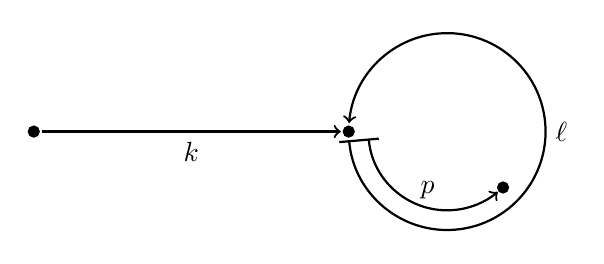
\begin{tikzpicture}
		\filldraw (-2, 0) circle (2pt); % Begin
		\draw[thick, ->] (-1.9, 0) -- node[below] {$k$} (1.9, 0) ;
		\filldraw (2, 0) circle (2pt); % End of k
		\draw[thick, |->] (3.25, 0) ++(-175:1.25) arc (-175:175:1.25);
		\node[xshift=4.7cm] {$\ell$};
		\draw[thick, |->] (3.25, 0) ++(-175:1) arc (-175:-50:1);
		\node[xshift=3cm, yshift=-0.75cm] {$p$};
		\filldraw (3.96, -0.71) circle (2pt);
	\end{tikzpicture}
	
	\caption{A description of how a path can be decomposed into a cycle, the path to it and a last part of it.}
	\label{PathDecompositionPrinciple}
\end{figure}

In the beginning we remarked that we have to fixate an alternation depth.
This bound can be seen in the definition of the transitive expansion and will be used in the logic that will characterise the Colour Refinement algorithm.
Therefore we can only reason about a fragment of $\GFC$, where the terms do not alternate too often.
This is formally stated in the following definition.

\begin{definition}[Alternation bounded $\GFC$]
	For a $k\in\mathbb N$, we define the fragment of $\GFC$ with a bounded alternation depth of $k$ ($\GFC_k$) as $\GFC$ with the constraint that for all formulae $\phi\in\GFC_k$ of signature $\sigma$ and every term $t$ that appears in $\phi$, there is an $n\in \mathbb{N}$ and an $\alpha\in \operatorname{Alters}_n^k(\sigma)$ such that $\alpha=t$.
	Atomic formulae are defined as usual, that is, the formulae $R(t_1(x_1),t_2(x_2),\dots,t_n(x_n))$ and $t_1(x_1)=t_2(x_2)$ for terms $t_1,t_2,\dots,t_n$ and variables $x_1,x_2,\dots,x_n$ are atomic formulae.
\end{definition}

With this, we can prove the first result, which allows us to use every $f^m(x)=y$ for every $m\in \mathbb N$ in a formula.

\begin{lemma}
	Let $\psi(x_1,x_2)\in \GFC_1$ be of the form $f^m(x_1)=x_2$. 
	Then there exists a formula $\theta(x_1,x_2)\in \GFC_1$ such that for any $\mathfrak A$ with $\vert \mathfrak A\vert=n$ it holds
	$$\mathfrak A,a_1,a_2 \models \psi(x_1,x_2) \text{ if, and only if, } \mathfrak A,a_1,a_2 \models \theta(x_1,x_2)$$ 
	and for any $f^{m'}(x)$ that appears in $\theta$ we have $m'\leq n$.
	Furthermore, $\theta(x_1,x_2)$ is of the form $\bigvee \Phi(x_1,x_2)$, and if $\mathfrak A,a_1,a_2\models \theta(x_1,x_2)$, then there is exactly one $\phi(x_1,x_2)\in\Phi$, such that $\mathfrak A,a_1\models \exists^{\geq 1} x_2 . \phi(x_1,x_2)$.
	\label{Simple_fm_to_fk}
\end{lemma}
\begin{proof}
	If $m \leq n$, we let $\theta\coloneqq\psi$ and the claim follows.
	
	Otherwise, we define
	$$\theta(x_1,x_2)\coloneqq \bigvee_{(k,\ell,p)\in \mathcal I(n,m)} \zeta_{(k,\ell,p)}(x_1,x_2)$$
	where
	\begin{align*}
		\zeta_{(k,\ell,p)}(x_1,x_2)\coloneqq & f^{k+p}(x_1)=x_2 \land f^{k}(x_1)=f^{k+\ell}(x_1) \\
		& \land \operatorname{E}^{k,\ell}_{f}(x_1)  \\
		& \land \bigwedge_{\ell'<\ell}f^{k}(x_1)\neq f^{k+\ell'}(x_1)
	\end{align*}
	and for some term $t(x_1)$ we have
	$$\operatorname{E}^{k,\ell}_{f}(t(x_1))=\begin{cases}
		\top & \text{if } k=0 \\
		f^{k-1}(t(x_1))\neq f^{k-1+\ell}(t(x_1)) & \text{otherwise}.
	\end{cases}$$
	Due to the definition of $\mathcal I(n,m)$ it is obvious that only $f^{m'}$ with $m'\leq n$ appears.
	We now proceed to the proof of the equivalence.
	For the purpose of readability, we will write $f_{\mathfrak A}$ instead of $f^{\mathfrak A}$.
	
	We will show that if $\mathfrak A,a_1,a_2 \models \theta(x_1,x_2)$, then $\mathfrak A,a_1,a_2 \models \psi(x_1,x_2)$.
	Let $\mathfrak A,a_1,a_2 \models \theta(x_1,x_2)$. 
	By definition of $\theta$, there are $(k,\ell,p)\in \mathcal I(n,m)$ with $\mathfrak A,a_1,a_2 \models \zeta_{(k,\ell,p)}(x_1,x_2)$.
	In particular $f_{\mathfrak A}^{k}(a_1)=f_{\mathfrak A}^{k+\ell}(a_1)$. It follows that
	$$f_{\mathfrak A}^{k}(a_1)=f_{\mathfrak A}^{k+\ell}(a_1)=f_{\mathfrak A}^{k+2\ell}(a_1)=f_{\mathfrak A}^{k+3\ell}(a_1) = \dots = f_{\mathfrak A}^{k+r\cdot \ell}(a_1)$$
	for all $r\in \mathbb N$. By using the definition of $\mathcal{I}(n,m)$, we get
	$$a_2 =f_{\mathfrak A}^{k+p}(a_1) = f_{\mathfrak A}^{k+r\cdot \ell + p}(a_1)=f_{\mathfrak A}^{m}(a_1).$$
	From this we can deduce $\mathfrak A,a_1,a_2\models \psi(x_1,x_2)$, where $\psi(x_1,x_2)$ has the form $f^{m}(x_1)=x_2$.
	
	Now we prove that if $\mathfrak A,a_1,a_2 \models \psi(x_1,x_2)$, then $\mathfrak A,a_1,a_2 \models \theta(x_1,x_2)$. 
	Let $\mathfrak A,a_1,a_2\models \psi(x_1,x_2)$. By assumption $m>n$ and by the pigeonhole principle there have to be distinct $i$ and $j$ such that $f_{\mathfrak A}^{i}(a_1)=f_{\mathfrak A}^{j}(a_1)$.
	Choose such $i$, $j$ such that they are lexicographically minimal.
	Now choose $k\coloneqq i$, $\ell \coloneqq j-i$ and $p\coloneqq (m-i) \mod (j-i)= (m-i) \mod \ell$.
	Obviously $(k,\ell,p)\in\mathcal I(n,m)$ and what remains to be shown is that $\mathfrak A,a_1,a_2\models \zeta_{(k,\ell,p)}(x_1,x_2)$.
	For that, we consider the parts of the conjunction and show for each one that it is satisfied.
	
	\begin{itemize}
		\item $f^{k+p}(x_1)=x_2$ is satisfied.
		We use the fact that $a= b \mod c \Leftrightarrow b = r\cdot c +a \text{ for some } r\in \mathbb N$.
		Then
		$$f_{\mathfrak A}^{k+p}(a_1)=f_{\mathfrak A}^{i+(m-i)-r\cdot \ell}(a_1)=f_{\mathfrak A}^{i+r\cdot \ell + m -i - r\cdot \ell}(a_1)=f_{\mathfrak A}^{m}(a_1)=a_2.$$
		Therefore $\mathfrak A,a_1,a_2\models f^{k+p}(x_1)=x_2$.
		
		\item $f^{k}(x_1)=f^{k+\ell}(x_1)$ is satisfied.
		Consider that
		$$f_{\mathfrak A}^{k}(a_1)=f_{\mathfrak A}^{i}(a_1)=f_{\mathfrak A}^{j}(a_1)=f_{\mathfrak A}^{j+i-i}(a_1)=f_{\mathfrak A}^{i+j-i}(a_1)=f_{\mathfrak A}^{k+\ell}(a_1).$$
		This leads to $\mathfrak A,a_1,a_2\models f^{k}(x_1)=f^{k+\ell}(x_1)$.
		
		\item $\operatorname{E}^{k,\ell}_f(x_1)$ is satisfied.
		Otherwise $f_{\mathfrak A}^{k-1}(a_1)=f_{\mathfrak A}^{k-1+\ell}(a)$, but then $(k-1,\ell)$ would be lexicographically smaller than $(i,j)$.
		
		\item The same reasoning applies to $\bigwedge_{\ell'<\ell}f^{k}(x_1)\neq f^{k+\ell'}(x_1)$. 
		If it weren't satisfied, there would be a $(i,j')$ with $j'<j$ and $f_{\mathfrak A}^{i}(a_1)=f_{\mathfrak A}^{i+j'}(a_1)$ which would be lexicographically smaller than $(i,j)$.
	\end{itemize}
	
	Thus we have shown that every subformula of the conjunction and therefore the formula is being fulfilled.
	
	Lastly, it remains to prove that if $\theta$ is satisfied, then there is exactly one $(k,\ell,p)\in\mathcal{I}(n,m)$ such that $\exists^{\geq 1}x_2.\zeta_{(k,\ell,p)}(x_1, x_2)$ is fulfilled.
	We prove this by contradiction.
	Assume that $\mathfrak A,a_1,a_2\models \theta(x_1,x_2)$ and that there are $\zeta_{(k,\ell,p)}(x_1,x_2)$ and $\zeta_{(k',\ell',p')}(x_1,x_2)$ with $(k,\ell,p)\neq (k',\ell',p')$, such that $\mathfrak A,a_1\models \exists^{\geq 1}x_2.\zeta_{(k,\ell,p)}(x_1,x_2)$ and $\mathfrak A,a_1\models \exists^{\geq 1}x_2.\zeta_{(k',\ell',p')}(x_1,x_2)$.
	
	We proceed with a case distinction. 
	Let $k=k'$ and $\ell=\ell'$.
	Then there are $r,r'\in\mathbb N$ such that
	$$k+r\cdot \ell + p = k'+r'\cdot \ell' + p'=m.$$
	Thus we can infer that $r\cdot \ell+p = r'\cdot \ell'+p'$.
	By definition of $\mathcal{I}(n,m)$ we know that $p,p'<\ell=\ell'$ and as such 
	$$r\cdot \ell +p,r'\cdot \ell'+p'\in \{r\cdot \ell,r\cdot \ell +1,\dots, r\cdot \ell +(\ell-1)\}$$
	and because $p$ is a non-negative integer, $r=r'$ has to follow and further we get $p=p'$.
	However this would contradict that $(k,\ell,p)\neq (k',\ell',p')$.
	Now assume that $\ell\neq\ell'$ and without loss of generality assume that $\ell<\ell'$.
	But then $\mathfrak A,a_1 \not\models \bigwedge_{\hat{\ell}<\ell'}f^{k'}(x_1)\neq f^{k'+\hat{\ell}}(x_1)$, because 
	$$f^{k'+\ell}_{\mathfrak A}(a_1)=f^{k+\ell}_{\mathfrak A}=f^k_{\mathfrak A}(a_1)=f^{k'}_{\mathfrak A}(a_1)$$
	and $k'+\ell < k'+\ell'$.
	Thus this cannot be the case as well.
	
	Consider that $k\neq k'$ and without loss of generality assume that $k<k'$.
	If $\ell=\ell'$, then by the principle of induction, we get that $f_{\mathfrak A}^k(a_1)=f_{\mathfrak A}^{k+\ell}(a_1)$, $f_{\mathfrak A}^{k+1}(a_1)=f_{\mathfrak A}^{k+1+\ell}(a_1)$ and then $f_{\mathfrak A}^{k'}(a_1)=f_{\mathfrak A}^{k'+\ell'}(a_1)$.
	But this contradicts $\mathfrak A,a_1 \models \operatorname{E}^{k',\ell'}_f(x_1)$.
	If $\ell < \ell'$, then 
	$$f_{\mathfrak A}^{k'}(a_1) =f_{\mathfrak A}^{k+(k'-k)}(a_1)=f_{\mathfrak A}^{k+(k'-k)+\ell}(a_1) = f_{\mathfrak A}^{k'+\ell}(a_1),$$
	but this again contradicts $\mathfrak A,a_1 \models \bigwedge_{\hat{\ell}<\ell'}f^{k'}(x_1)\neq f^{k'+\hat{\ell}}(x_1)$.
	If $\ell'<\ell$, then there exists a $t\in\mathbb N$ such that 
	$$k+t\cdot  \ell < k' \leq k+(t+1)\cdot \ell.$$
	We now define $r\coloneqq k+(t+1)\cdot \ell -k'$ and get $f_{\mathfrak A}^{k'+r}(a_1)=f_{\mathfrak A}^{k'+r+\ell'}$ and by using $f_{\mathfrak A}^{k'+r}(a_1)=f_{\mathfrak A}^{k+(t+1)\cdot \ell}(a_1)=f_{\mathfrak A}^k(a_1)$ it follows that $f_{\mathfrak A}^{k}(a_1)=f_{\mathfrak A}^{k+\ell'}(a_1)$.
	This contradicts $\mathfrak A,a_1 \models \bigwedge_{\hat{\ell}<\ell}f^{k}(x_1)\neq f^{k'+\hat{\ell}}(x_1)$.
	
	One can see that we did not use $x_2$ or $a_2$.
	Therefore its interpretation is irrelevant, which is why we can existentially quantify it in the claim.
	As all possible cases lead to a contradiction, the first assumption cannot be true and we proved the claim.
\end{proof}

The above proof allows for the translation of a formula $f^m(x)=y$ to a formula $\theta(x,y)$ that is equivalent for structures with $n$ elements.
A natural extension would be, to allow alternation of functions, for example formulae like $g^m(f^{m'}(x))=y$.
This is also possible and will be proved in the following.

\begin{lemma}
	Let $d\in\mathbb N$ and $\psi(x_1,x_2)\in \GFC_d$ be of the form $t(x_1)=x_2$ for a term $t$.
	Then there exists a formula $\theta_{t}(x_1,x_2)\in\GFC_d$, such that for any structure $\mathfrak A$ with $\vert \mathfrak A \vert = n$ it holds
	$$\mathfrak A,a_1,a_2 \models \psi(x_1,x_2) \text{ if, and only if, } \mathfrak A,a_1,a_2 \models \vartheta_{t}(x_1,x_2).$$ 
	Furthermore, $\theta_{t}(x_1,x_2)$ is of the form $\bigvee \Phi(x_1,x_2)$ where all $\phi(x_1,x_2)\in\Phi(x_1,x_2)$ are of the form
	$$t'(x_1)=x_2 \land \bigwedge \Psi(x_1)$$ 
	for some term $t'(x_1)$, and for every function symbol $f$ in the signature, there does not appear a term of the form $f^m(s(x))$ where $m > n$.
	Additionally, if $\mathfrak A,a_1,a_2\models \theta_{t}(x_1,x_2)$, then there is exactly one $\phi\in\Phi$, such that $\mathfrak A,a_1\models \exists^{\geq 1}x_2.\phi(x_1,x_2)$.
	\label{TranslationOfArbTerms}
\end{lemma}
\begin{proof}
	We prove this via an induction on the term $t(x_1)$.
	
	\textbf{Base case:}
	If $t(x_1)$ is of the form $f^{m}(x_1)$ for a unary function symbol $f$ and $m\in \mathbb N$, we use the formula constructed in the proof of \cref{Simple_fm_to_fk}.
	It can easily be verified that it is in the correct form and from the same proof we get that if the translated formula is fulfilled, exactly one subformula of the disjunction is satisfied.
	
	\textbf{Inductive step:}
	Assume that $t(x_1)$ is of the form $g^m(s(x_1))$ for a unary function symbol $g$, $m\in\mathbb N$ and term $s$.
	By the induction hypothesis, there is a formula $\theta_{s}(x_1,x_2)\in \GFC_{d-1}$ of the form $\bigvee \Phi_s(x_1,x_2)$ defined above with $\mathfrak A,a_1,a_2 \models s(x_1)=x_2$ if, and only if, $\mathfrak A,a_1,a_2\models \theta_{s}(x_1,x_2)$.
	
	If $m\leq n$, we set $\theta_{t}(x_1,x_2)$ to
	$$\bigvee \Phi'(x_1,x_2),$$
	where $\Phi'(x_1,x_2)\coloneqq\{g^{m}(t'(x_1))=x_2 \land \bigwedge \Psi(x_1) : t'(x_1)=x_2 \land \bigwedge \Psi(x_1)\in \Phi_s(x_1,x_2)\}$.
	
	If $m>n$, then we set $\theta_{t}(x_1,x_2)$ to
	$$\bigvee_{(k,\ell,p)\in \mathcal I(n,m)} \bigvee \Phi'_{(k,\ell,p)}(x_1,x_2),$$
	where 
	\begin{align*}
		\Phi'_{(k,\ell,p)}\coloneqq \{g^{k+p}(t'(x_1))=x_2 &\land g^{k}(t'(x_1))=g^{k+l}(t'(x_1)) \\
		& \land \operatorname{E}^{k,l}_g(t'(x_1)) \land \bigwedge_{\ell'<\ell} g^{k}(t'(x_1))\neq g^{k+\ell'}(t'(x_1)) \\
		& \land \Psi(x_1) : t'(x_1)=x_2 \land \bigwedge \Psi(x_1)\in \Phi_s(x_1,x_2)\}
	\end{align*}
	
	By using the above definitions, we get $\mathfrak A,a_1,a_2\models s(x_1)=x_2$ if, and only if, $\mathfrak A,a_1,a_2\models \phi_s(x_1,x_2)$ for some $\phi_s\in\Phi_s$ where $\phi_s(x_1,x_2)$ is of the form $t'(x_1)=x_2 \land \bigwedge \Psi(x_1)$.
	Therefore
	\begin{equation*}
		\mathfrak A, a_1,a_2 \models s(x_1)=x_2 \text{ if, and only if, } \mathfrak A,a_1,a_2 \models t'(x_1)=x_2 \land \bigwedge \Psi(x_1).
		\tag{$\star$}
		\label{eq:a}
	\end{equation*}
	
	We now prove that 
	$$\mathfrak A, a_1,a_2\models t(x_1)=x_2 \text{ if, and only if, } \mathfrak A,a_1,a_2\models \theta_{t}(x_1,x_2).$$
	Assume $m\leq n$.
	Let $\mathfrak A, a_1,a_2 \models \theta_{t}$.
	Then there is some $\phi(x_1,x_2)$ of the form $g^{m}(t'(x_1))=x_2 \land \bigwedge \Psi(x_1)$ such that $\mathfrak A,a_1,a_2\models \phi(x_1,x_2)$.
	We then get
	\begin{align*}
		\mathfrak A,a_1,a_2 \models & g^{m}(t'(x_1))=x_2 \land \bigwedge \Psi(x_1) \\
		\Leftrightarrow \mathfrak A,a_1,a_2,a_3 \models & g^{m}(x_3)=x_2 \land \bigwedge \Psi(x_1) \land t'(x_1)=x_3 \text{ for some } a_3\in A \\
		\overset{(\star)}{\Leftrightarrow} \mathfrak A,a_1,a_2,a_3\models & g^{m}(x_3)=x_2 \land s(x_1)=x_3 \text{ for some } a_3\in A \\
		\Leftrightarrow \mathfrak A,a_1,a_2 \models & g^{m}(s(x_1))=x_2.
	\end{align*}
	
	Now let $m>n$.
	Then there is a
	\begin{align*}
		\phi(x_1,x_2)\coloneqq g^{k+p}(t'(x_1))=x_2 &\land g^{k}(t'(x_1))=g^{k+l}(t'(x_1)) \\
		& \land \operatorname{E}^{k,l}_g(t'(x_1)) \land \bigwedge_{\ell'<\ell} g^{k}(t'(x_1))\neq g^{k+\ell'}(t'(x_1)) \\
		& \land \bigwedge \Psi(x_1)
	\end{align*}
	for some $(k,\ell,p)\in\mathcal I(n,m)$ with $\mathfrak A,a_1,a_2\models \phi(x_1,x_2)$.
	And now
	\begin{align*}
		\mathfrak A,a_1,a_2 \models & \phi(x_1,x_2) \\
		\Leftrightarrow A,a_1,a_2,a_3 \models &g^{k+p}(x_3)=x_2 \land g^{k}(x_3)=g^{k+l}(x_3) \\
		& \land \operatorname{E}^{k,l}_g(x_3) \land \bigwedge_{\ell'<\ell} g^{k}(x_3)\neq g^{k+\ell'}(x_3) \\
		& \land \bigwedge\Psi(x_1) \land t'(x_1)=x_3 \text{ for some } a_3\in A \\
		\overset{\ref{Simple_fm_to_fk}}{\Leftrightarrow} \mathfrak A, a_1,a_2,a_3 \models & g^{m}(x_3)=x_2 \land t'(x_1)=x_3 \land \bigwedge\Psi(x_1) \text{ for some } a_3 \in A \\
		\overset{(\star)}{\Leftrightarrow} \mathfrak A,a_1,a_2,a_3 \models & g^{m}(x_3)=x_2\land s(x_1)=x_3 \text{ for some } a_3\in A \\
		\Leftrightarrow \mathfrak A,a_1,a_2 \models & g^{m}(s(x_1))=x_2.
	\end{align*}
	The other direction follows in both cases, as only equivalent steps have been used and it is obvious that the disjunction of a set is being fulfilled, if a formula of the set is satisfied.
	
	Lastly, we show that if $\mathfrak A,a_1,a_2\models \theta_t(x_1,x_2)$, where $\theta_t$ is of the form $\bigvee \Phi$, there is exactly one $\phi\in\Phi$, such that $\mathfrak A,a_1\models \exists^{\geq 1} x_2.\phi(x_1,x_2)$.
	As in the proof of \cref{Simple_fm_to_fk}, we are going to use a proof by contradiction and we will look at the cases where $m\leq n$ and $m> n$ separately.
	If $m\leq n$, assume that $\mathfrak A,a_1,a_2\models \theta_t(x_1,x_2)$ and that there are $\phi_1,\phi_2\in \Phi'(x_1,x_2)$ with $\phi_1\neq \phi_2$, $\mathfrak A,a_1\models \exists^{\geq 1}x_2.\phi_1(x_1,x_2)$ and $\mathfrak A,a_1\models \exists^{\geq 1}x_2.\phi_2(x_1,x_2)$.
	It is easy to see that 
	$$\mathfrak A,a_1,a_2,a_3\models g^m(t'_1(x_1))=x_2 \land \bigwedge \Psi_1(x_1) \land g^m(t'_2(x_1))=x_3 \land \bigwedge\Psi_2(x_1)$$
	for some $a_2$ and $a_3$, which is equivalent to
	\begin{align*}
		\mathfrak A,a_1,a_2,a_3,a_4,a_5\models
		\phantom{\land} &g^m(x_4)=x_2 \land t'_1(x_1)=x_4\land \bigwedge\Psi_1(x_1) \\ 
		\land &g^m(x_5)=x_3 \land t'_2(x_1)=x_4 \land \bigwedge\Psi_2(x_1)
	\end{align*}
	for some $a_4$ and $a_5$.
	However, $t'_1(x_1)=x_2\land \bigwedge\Psi_1(x_1), t'_2(x_1)=x_s \land \bigwedge\Psi_2(x_1) \in \Phi_s$ and thus there would be
	two different $\psi_1(x_1,x_2),\psi_2(x_1,x_2)\in \Phi_s$ such that $\mathfrak A,a_1\models \exists^{\geq 1} x_2.\psi_1(x_1,x_2)$ and $\mathfrak A,a_1\models \exists^{\geq 1} x_2.\psi_2(x_1,x_2)$.
	But this contradicts the induction hypothesis that $\Phi_s$ conforms to the properties stated in the lemma.
	
	If $m>n$, we again assume that $\mathfrak A,a_1,a_2\models \theta_t(x_1,x_2)$ and that there are $\phi_1(x_1,x_2)\in\Phi'_{(k,\ell,p)}(x_1,x_2)$ and $\phi_2(x_1,x_2)\in\Phi'_{(k',\ell',p')}(x_1,x_2)$ with $\phi_1\neq \phi_2$, $\mathfrak A,a_1\models \exists^{\geq 1}x_2.\phi_1(x_1,x_2)$ and $\mathfrak A,a_1\models \exists^{\geq 1}x_2.\phi_2(x_1,x_2)$.
	By looking at the structure of the formulae as they are defined in this proof and by substituting terms and variables like in the first case, we again find that 
	$$\mathfrak A,a_1,a_3,a_4\models t'_1(x_1)=x_3\land \bigwedge\Psi_1(x_1) \land t'_2(x_1)=x_4 \land \bigwedge\Psi_2(x_1),$$
	where $t'_1(x_1)=x_2\land\bigwedge \Psi_1(x_1), t'_2(x_1)=x_2\land\bigwedge \Psi_2(x_1)\in \Phi_s$.
	By using the same arguments as before, we as well arrive at a contradiction.
	As such, the assumption must be false and we have finished the proof.
\end{proof}

Finally, we want to be able to use terms inside relations.
This is also possible and will be shown in the following lemma.

\begin{lemma}
	Let $d\in\mathbb N$ and $\psi(x_1,\dots,x_m)\coloneqq R(t_1(x_1),\dots,t_m(x_m))\in \GFC_d$ be an atomic formula.
	Then there exists a formula $\theta_\psi\in\GFC_d$, such that for any given structure (of fitting signature) $\mathfrak A$ with $\vert\mathfrak A \vert=n$ it holds
	$$\mathfrak A,a_1,\dots,a_m\models \psi(x_1,\dots,x_m) \text{ if, and only if, } \mathfrak A,a_1,\dots,a_m\models \theta_\psi(x_1,\dots,x_m).$$
	Furthermore, $\theta_\psi(x_1,\dots,x_m)$ is of the form $\bigvee \Phi(x_1,\dots,x_m)$ where all $\phi\in\Phi$ are of the form
	$$R(t_1'(x_1),\dots,t_m'(x_m))\land \bigwedge\Psi_1(x_1)\land \dots\land\bigwedge \Psi_m(x_m),$$
	and for every $f^m(s(x))$ that appear in $\theta_\psi$, where $f$ is a unary function symbol and $s$ is a term we have $m\leq n$.
	Additionally, if $\mathfrak A,a_1,\dots,a_m\models \theta_\psi(x_1,\dots,x_m)$, then there exists exactly one $\phi(x_1,\dots,x_m)\in\Phi(x_1,\dots,x_m)$, such that $\mathfrak A,a_1,\dots,a_m\models \phi(x_1,\dots,x_m)$.
	\label{TranslationOfArbAtomics}
\end{lemma}
\begin{proof}
	Let $\mathfrak A,a_1,\dots,a_m\models\psi(x_1,\dots,x_m)$.
	This is equivalent to 
	$$\mathfrak A,a_1,\dots,a_m,b_1,\dots,b_m\models R(b_1,\dots,b_m)\land t_1(x_1)=b_1\land\dots\land t_m(x_m)=b_m$$
	for some $b_1,\dots,b_m\in A$.
	By applying the previous lemma, we get the equivalent statement
	\begin{align*}
		\mathfrak A,a_1,\dots,a_m,b_1,\dots,b_m\models R(y_1,\dots,y_m) \land& \bigvee_{i_1}\left(t_{1,i_1}'(x_1)=y_1\land \bigwedge\Psi_{1,i_1}(x_1)\right) \\
		\land& \dots \\
		\land& \bigvee_{i_m}\left(t_{m,i_m}'(x_m)=y_m\land \bigwedge\Psi_{m,i_m}(x_m)\right).
	\end{align*}
	Through distribution of boolean formulae we get
	\begin{align}
		\mathfrak A,a_1,\dots,a_m,b_1,\dots,b_m\models \bigvee_{i_1} \dots \bigvee_{i_m} ( R(y_1,\dots,y_m)\land & t_{1,i_1}'(x_1)=y_1 \land \bigwedge\Psi_{1,i_1}(x_1) \nonumber \\
		\land & \dots \label{EquivalentDistributedAtomic}\\
		\land & t_{m,i_m}'(x_m)=y_m \land \bigwedge\Psi_{m,i_m}(x_m) ). \nonumber
	\end{align}
	Finally, we can resubstitute variables and get
	\begin{align*}
		\mathfrak A,a_1,\dots,a_m\models \bigvee_{i_1}\dots\bigvee_{i_m} &(R(t_{1,i_1}'(x_1),\dots,t_{m,i_m}'(x_m)) \\
		&\land \bigwedge\Psi_{1,i_1}(x_1) \\
		&\land\dots \\
		&\land\bigwedge\Psi_{m,i_m}(x_m))\eqqcolon \theta_\psi(x_1,\dots,x_m).
	\end{align*}
	One can see that $\theta_\psi$ is of the correct form.
	The equality follows from the fact that only equivalences have been used to derive $\theta_\psi$ from $\psi$.
	
	Lastly, we prove that if $\theta_\psi$ is satisfied, there is exactly one formula of the disjunction that is satisfied.
	For this, consider the equivalent formula from \cref{EquivalentDistributedAtomic}.
	Assume that $\mathfrak A,a_1,\dots,a_m\models \theta_\psi$ and that there are two subformulae $\phi_1$ and $\phi_2$ of the formula in \cref{EquivalentDistributedAtomic}, where $\phi_1$ is of the form 
	\begin{align*}
		R(y_1,\dots,y_m)\land & t_{1,i_1}'(x_1)=y_1 \land \bigwedge\Psi_{1,i_1}(x_1) \\
		\land & \dots \\
		\land & t_{m,i_m}'(x_m)=y_m \land \bigwedge\Psi_{m,i_m}(x_m)
	\end{align*}
	and $\phi_2$ is of the form
	\begin{align*}
		R(y_1,\dots,y_m)\land & s_{1,i_1}'(x_1)=y_1 \land \bigwedge\Psi'_{1,i_1}(x_1) \\
		\land & \dots \\
		\land & s_{m,i_m}'(x_m)=y_m \land \bigwedge\Psi'_{m,i_m}(x_m),
	\end{align*}
	such that $\phi_1\neq\phi_2$, $\mathfrak A,a_1,\dots,a_m,b_1,\dots,b_m\models \phi_1$ and $\mathfrak A,a_1,\dots,a_m,b_1,\dots,b_m\models \phi_2$.
	As $\phi_1\neq \phi_2$, there must be a $j$ such that $\psi_1$ is of the form $t'_{j,i_j}(x_j)=y_j\land \bigwedge \Psi_{j,i_j}(x_j)$, $\psi_2$ is of the form $s'_{j,i_j}(x_j)=y_j\land\bigwedge \Psi'_{j,i_j}(x_j)$ and $\psi_1\neq\psi_2$.
	From the construction of the formula we know, that there is a term $t_j$, a formula $\theta_{t_j}$ of the form $\bigvee \Phi_{t_j}$ and $\psi_1,\psi_2\in\Phi_{t_j}$.
	However, $\mathfrak A,a_j\models \exists^{\geq 1}y_j . \psi_1(x_j,y_j)$ and $\mathfrak A,a_j\models \exists^{\geq 1}y_j.\psi_2(x_j,y_j)$ would contradict the claim that has been proved in \cref{TranslationOfArbTerms}.
\end{proof}

To illustrate how this translation works, let us consider the formula $\psi$ of the form $g^4(f^3(x))=y$ for a structure with $2$ elements.
As in the proof, we inductively translate the inner terms and as such get for the formula $f^3(x)=y$, the formula $\phi$ of the form
$$\bigvee_{(k,\ell,p)\in \mathcal I(2,3)}\left(f^k(x)=f^{k+\ell}(x)\land f^{k+p}(x)=y \land \operatorname{E}^{k,l}_f(x)\land\bigwedge_{\hat \ell < \ell} f^k(x)\neq f^{k+\hat\ell}(x)\right)$$
and with $\mathcal I(2,3)=\{(0,2,1),(1,1,0),(0,1,0)\}$ we get that $\phi$ equals
\begin{align*}
	\phantom{\lor}&\left(x=f^2(x) \land f(x)=y \land x\neq f(x)\right) \\
	\lor & \left(f(x)=f^2(x) \land f(x)=y \land x \neq f(x)\right) \\
	\lor & \left(x=f(x) \land x=y \land \top\right).
\end{align*}
Now we can construct $\theta_\psi$ from $\psi$. 
From the proof, we know that $\theta_\psi$ is of the form
\begin{align*}
	\bigvee_{(k',\ell',p')\in \mathcal I(2,4)}\bigvee_{(k,\ell,p)\in \mathcal I(2,3)} (
	&f^k(x)=f^{k+\ell}(x)\land \operatorname{E}^{k,l}_f(x)\land\bigwedge_{\hat{\ell}<\ell}f^k(x)\neq f^{k+\hat\ell}(x) \\
	& \land g^{k'}(f^{k+p}(x))=g^{k'+\ell'}(f^{k+p}(x)) \land g^{k'+p'}(f^{k+p}(x)) = y \\
	& \land E^{k',\ell'}_g(f^{k+p}(x)) \land \bigwedge_{\hat{\ell}<\ell'}g^{k'}(f^{k+p}(x))\neq g^{k'+\hat\ell}(f^{k+p}(x)))
\end{align*}
and with $\mathcal I(2,4)=\{(1,1,0),(0,1,0), (0,2,0)\}$ we find $\theta_\psi$ analogously.

This now allows us to prove the logical characterisation of our Colour Refinement Algorithm.

\begin{theorem}
	\label{thm:ThmB}
	Let $\mathfrak A$ and $\mathfrak B$ be two structures of the same signature $\sigma$ with relation and unary function symbols and let $k\in \mathbb{N}$.
	Then the two following statements are equivalent:
	\begin{enumerate}
		\item $\RCR_k$ distinguishes $\mathfrak A$ and $\mathfrak B$.
		\item There exists a sentence $\phi\in\GFC_k$ such that $\mathfrak A\models \phi$ and $\mathfrak B\not\models \phi$.
	\end{enumerate}
\end{theorem}
\begin{proof}
	We prove that \emph{1.} implies \emph{2.}. 
	Let $\mathfrak A$ and $\mathfrak B$ be distinguished by $\RCR_k$.
	If they are of different sizes, assume without loss of generality that 
	$$\vert \mathfrak A \vert =n > n'=\vert \mathfrak B \vert.$$
	Then define $\phi\coloneqq \exists^{\geq n} x. \top\in \GFC_k$, which obviously distinguishes the structures.
	
	Now assume $\vert \mathfrak A\vert = \vert \mathfrak B \vert = n$.
	By definition, $\RCR$ distinguishes $\widetilde{\mathfrak A}$ and $\widetilde{\mathfrak B}$.
	When using the proof from \cite{scheidt2025ColorRefinement}, we obtain a formula $\widetilde{\phi}\in \GFC$ of signature $\widetilde{\sigma}$ that distinguishes the expansions.
	This formula $\widetilde{\phi}$ can then be translated to a formula $\phi\in\GFC_k$ of signature $\sigma$.
	Replace every atomic subformula $\operatorname{Eq}_{\alpha,\beta}(x,y)$, where $\alpha,\beta\in \operatorname{Alters}_n^k(\sigma)$,  by the formula $\alpha(x)=\beta(y)$.
	Similarly, replace every atomic subformula $R_{\alpha_1,\dots,\alpha_\ell}(x_1,\dots,x_\ell)$ by the formula $R(\alpha_1(x_1),\dots,\alpha_\ell(x_\ell))$.
	Obviously, if a structure's expansion satisfied $\widetilde{\phi}$, it also satisfies $\phi$ and vice versa.
	Therefore, we get a formula $\phi\in \GFC_k$ that distinguishes $\mathfrak A$ and $\mathfrak B$.
	
	Now we prove that \emph{2.} implies \emph{1.}.
	Let $\phi\in \GFC_k$ such that $\mathfrak A\models \phi$ and $\mathfrak B\not\models \phi$.
	Using \cref{TranslationOfArbAtomics} we can obtain a formula $\theta_\psi$ for every atomic subformula $\psi$ of $\phi$ with $\mathfrak A\models \psi$ if, and only if, $\mathfrak A\models \theta_\psi$.
	With this we can construct an equivalent formula $\phi'\in\GFC_k$, which then allows us, to easily translate it to $\widetilde{\sigma}$.
	We will construct this formula $\phi'$ inductively and directly prove the equivalence.
	
	\begin{claim}
		The two formulae $\phi$ and $\phi'$ are equivalent.
	\end{claim}
	\begin{proof}
		\textbf{Base cases:}
		If $\phi$ is an atomic formula, that is, either a term equivalence or a relation, then set $\phi'$ to $\theta_\phi$.
		The equivalence follows directly from the above Lemmas \ref{TranslationOfArbTerms} and \ref{TranslationOfArbAtomics}.
		
		\textbf{Inductive cases:}
		In the cases where $\phi$ is of the form $\neg\theta$ or $\theta_1\land\theta_2$, we set $\phi'$ to $\neg\theta'$ or $\theta_1'\land\theta_2'$ and the claim follows directly using the induction hypothesis.
		
		Let $\phi$ be of the form $\exists^{\geq\ell}\mathbf v. \Delta\land \theta$.
		In addition to translating $\Delta$ and $\theta$ to $\theta_\Delta$ and $\theta'$, respectively, we also will need to transform the formula, so that it still is a valid formula in $\GFC_k$.
		When looking at the possible translations from the atomic formula $\Delta(x_1,\dots,x_m)$, we see that it must be of the form $\bigvee_{i\in[o]} (\Delta'_i(x_1,\dots,x_m) \land \bigwedge \Psi_i(x_1,\dots,x_m))$.
		When considering the transformed formula 
		$$\exists^{\geq \ell}\mathbf v. \left(\bigvee_{i\in [o]}\left(\Delta'_i\land\bigwedge \Psi_i\right) \land \theta'\right),$$
		we then will distribute $\theta'$ over the disjunction and thus define
		$$\psi \coloneqq \exists^{\geq \ell}\mathbf v. \left(\bigvee_{i\in[o]} \left(\Delta'_i\land\bigwedge \Psi_i \land \theta'\right)\right)$$
		In the following we prove the equivalence of $\phi$ and $\psi$.
		Let $\mathfrak A\models \phi$.
		This means there are at least $\ell$ tuples $\mathbf a\in A$, such that $(\mathfrak A,\mathbf a)\models \Delta(\mathbf v) \land \theta(\mathbf v)$.
		Using the induction hypothesis we get that this is equivalent to $(\mathfrak A,\mathbf a)\models \bigvee(\Delta'\land\bigwedge\Psi)\land \theta'$, which, using the distributive law of propositional logic, is equivalent to $(\mathfrak A,\mathbf a)\models \bigvee(\Delta'\land\bigwedge\Psi\land\theta')$.
		Therefore the number of tuples that satisfy $\Delta\land\theta$ must be the same as for $\bigvee(\Delta'\land\bigwedge\Psi\land\theta')$ and $\mathfrak A\models \exists^{\geq\ell}\mathbf v. \bigvee (\Delta'\land\bigwedge\Psi\land\theta')$ follows.
		
		However, we are not finished, because $\psi \notin \GFC_k$.
		We will solve this, by considering all possible segmentations of the disjunction.
		Informally, for $o,\ell\in\mathbb N$ we define $\operatorname{Parts}(o, \ell)$ as the set of all multisets with exactly $\ell$ elements of $[o]$, respecting their multiplicity.
		We then define $\phi'$ as
		$$\bigvee_{(M,\operatorname{mult}_M)\in \operatorname{Parts}(o,\ell)} \bigwedge_{i\in M} \exists^{\geq \operatorname{mult}_M(i)}\mathbf v. (\Delta'_i\land\bigwedge \Psi_i \land \theta')$$
		and will prove the equivalence between $\psi$ and $\phi'$ in the following. 
		
		Let $\mathfrak A\models \psi$.
		Then there are $\ell$ different tuples $\mathbf a$, such that $\mathfrak A,\mathbf a \models \bigvee_{i\in[o]}(\Delta'_i\land\bigwedge\Psi_i\land\theta')$.
		From the above lemmas we know that for every such tuple, there is exactly one $i$ such that $\mathfrak A,\mathbf a\models \Delta'_i\land\bigwedge \Psi_i\land \theta'$.
		Now construct a multiset $(M,\operatorname{mult}_M)$ with exactly these $i$ that are being satisfied and with the multiplicity of the amount of tuples satisfying them.
		One can see that $(M,\operatorname{mult}_M)\in \operatorname{Parts}(o,n)$ and that 
		$$\mathfrak A \models \bigwedge_{i\in M}\exists^{\geq\operatorname{mult}_M(i)}\mathbf v. (\Delta'_i\land \bigwedge\Psi_i\land \theta').$$
		It directly follows that $\mathfrak A\models \phi'$.
		
		Let $\mathfrak A\models \phi'$.
		From the construction we know, that every $\mathbf a$ that is being quantified satisfies only the $\Delta'_i\land\bigwedge\Psi_i\land\theta'$ they are being quantified for.
		By the definition of $\operatorname{Parts}(o,\ell)$, we thus get exactly $\ell$ tuples that satisfy some $\Delta'_i\land\bigwedge\Psi_i\land\theta'$ and $\mathfrak A\models \psi$ follows.
		We therefore have proved the claim.
	\end{proof}
	
	Note that for every term $\alpha$ that appears in $\phi'$, it holds that $\alpha\in \operatorname{Alters}^k_n(\sigma)$.
	This follows from the properties of the translation in \cref{TranslationOfArbAtomics}.
	Furthermore, for every atomic subformula, we have a corresponding relation symbol in $\widetilde{\sigma}$.
	With this, we can transform $\phi'$ to a formula $\widetilde{\sigma}\in\GFC$ of signature $\widetilde{\sigma}$, such that $\mathfrak A\models \phi'$ if, and only if, $\widetilde{\mathfrak A}\models \widetilde{\phi}$.
	
	It can be seen that the only subformulae that need to be changed are atomic.
	Let $\psi$ be an atomic formula that appears in $\phi'$.
	If $\psi$ is a term equation, that is, it is of the form $t(x)=s(y)$, we know through the construction of $\phi'$ and the definition of the transitive expansion, that there are $\alpha,\beta\in \operatorname{Alters}^k_n(\sigma)$ with $\alpha=t$ and $\beta=s$. 
	As such, we can replace $\psi$ with $\operatorname{Eq}_{\alpha,\beta}(x,y)$.
	
	If $\psi$ is a relation, that is, it is of the form $R(t_1(x_1),\dots,t_m(x_m))$, we again have $\alpha_1,\dots,\alpha_m\in \operatorname{Alters}^k_n(\sigma)$, such that $\alpha_i=t_i$ for $i\in[m]$.
	We then can replace $\psi$ with $R_{\alpha_1,\dots,\alpha_m}(x_1,\dots,x_m)$.
	From the semantic definition of the transitive expansion, it can be easily seen that $\mathfrak A\models \phi'$ if, and only if, $\widetilde{\mathfrak A}\models \widetilde{\phi}$.
	
	With this, we have obtained a formula $\widetilde{\phi}\in\GFC$ of signature $\widetilde{\sigma}$, where $\widetilde{\mathfrak A}\models \widetilde{\phi}$ and $\widetilde{\mathfrak B}\not\models \widetilde{\phi}$.
	Using \cite{scheidt2025ColorRefinement}, we thus know that $\RCR$ distinguishes $\widetilde{\mathfrak A}$ and $\widetilde{\mathfrak B}$ and by definition we can deduce that $\RCR_k$ distinguishes $\mathfrak A$ and $\mathfrak B$.
\end{proof}

We thus can characterise $\RCR_k$ with the logic $\GFC_k$.

\subsection{Characterisation Through Homomorphism Counting}
\label{sec:RCRwithFnHomCount}

One very interesting property of classical, as well as Relational Colour Refinement is that aside from its logical characterisation, it can be characterised by counting homomorphisms from certain structures.
As we showed, the logical characterisation of Relational Colour Refinement has two possible extensions to structures with functions.
Thus we now want to consider, whether those extensions can also be characterised by counting homomorphisms.

In the following we will see that, using the two established approaches, it is in general not possible, to find acyclic structures with functions that divide two structures by homomorphism count.
We will concentrate on the encoding defined in Section \ref{sec::NaiveEncodingOfFunctions}, where we will show one positive and one negative result.

To begin, let us define two concepts for relational structures that encode a non-relational structure.

\begin{definition}[Total structures]
	\label{def:TotalStructures}
	Let $\sigma\coloneqq \sigma_{\operatorname{Rel}} \operatorname{\dot{\cup}} \sigma_{\operatorname{Func}}$ be a signature where $\sigma_{\operatorname{Func}}$ contains exactly all function symbols and is not empty.
	Now let $\sigma'$ be the relational encoding of $\sigma$ and let $\mathfrak A'$ be a $\sigma'$-structure.
	We call $\mathfrak A'$ total, if for every $R_{f}\in\widehat{\sigma}$ with arity $n+1$ where $f\in \sigma_{\operatorname{Func}}$ has arity $n$, and every tuple $\mathbf x$ of length $n$, there is a $y$ such that $(\mathbf xy)\in R^{\mathfrak A'}_{f}$.
\end{definition}

Total structures therefore capture the notion that every relation that encodes a function is defined for the complete value-domain.
However, functions also only valuate to exactly one value.
This idea is captured by the following definition.

\begin{definition}[Functional structures]
	We define $\sigma$, $\sigma'$ and $\mathfrak A'$ exactly as in Definition \ref{def:TotalStructures}.
	We call $\mathfrak A'$ functional, if for every $R_{f}\in\widehat{\sigma}$ with arity $n+1$ where $f\in \sigma_{\operatorname{Func}}$ has arity $n$, we have that if $(\mathbf xy)\in R^{\mathfrak A'}_{f}$ there is no $y'\neq y$ such that $(\mathbf xy')\in R^{\mathfrak A'}_{f}$.
\end{definition}
\iffalse
A graphical representation of total and functional structures can be found in Figure \ref{fig:totalAndFunctionalStructs}.
\begin{figure}
	\centering
	\begin{subfigure}{0.49\textwidth}
		\centering
		\begin{tikzpicture}[node distance=4cm]
			\node[state] (a) {$a_1$};
			\node[state, right=of a] (b) {$a_2$};
			% \node[left=of a, xshift=2cm, yshift=1cm] (label) {$\mathfrak A$:};
			\draw 
			(a) edge[->, thick, above, bend left] node{$R_f$} (b)
			(b) edge[->, thick, below, bend left] node{$R_f$} (a);
		\end{tikzpicture}
		\caption{A total and functional structure.}
	\end{subfigure}
	\begin{subfigure}{0.49\textwidth}
		\centering
		\begin{tikzpicture}[node distance=4cm]
			\node[state] (a) {$b_1$};
			\node[state, right=of a] (b) {$b_2$};
			% \node[left=of a, xshift=2cm, yshift=1cm] (label) {$\mathfrak B$:};
			\draw 
			(a) edge[->, thick, above, bend left] node{$R_f$} (b)
			(b) edge[->, thick, below, bend left] node{$R_f$} (a)
			(a) edge[->, thick, loop left] node{$R_f$} (a);
		\end{tikzpicture}
		\caption{A total and not-functional structure.}
	\end{subfigure}
	\begin{subfigure}{0.49\textwidth}
		\centering
		\begin{tikzpicture}[node distance=4cm]
			\node[state] (a) {$c_1$};
			\node[state, right=of a] (b) {$c_2$};
			% \node[left=of a, xshift=2cm, yshift=1cm] (label) {$\mathfrak C$:};
			\draw 
			(a) edge[->, thick, above, bend left] node{$R_f$} (b);
		\end{tikzpicture}
		\caption{A not-total, but functional structure.}
	\end{subfigure}
	\begin{subfigure}{0.49\textwidth}
		\centering
		\begin{tikzpicture}[node distance=4cm]
			\node[state] (a) {$d_1$};
			\node[state, right=of a] (b) {$d_2$};
			% \node[left=of a, xshift=2cm, yshift=1cm] (label) {$\mathfrak D$:};
			\draw 
			(a) edge[->, thick, above, bend left] node{$R_f$} (b)
			(a) edge[->, thick, loop left] node{$R_f$} (a);
		\end{tikzpicture}
		\caption{A not-total and not-functional structure.}
	\end{subfigure}
	\caption{Examples for different combinations of total and functional structures with $\sigma=\{f/1\}$ and thus $\sigma'=\{R_f/2\}$.}
	\label{fig:totalAndFunctionalStructs}
\end{figure}
\fi
To continue, we have to define what it means to be acyclic for a structure with functions.

\begin{definition}[Acyclic, non-relational structures]
	Let $\sigma$ be a signature with function symbols and $\sigma'$ its encoding as it is defined in Section \ref{sec::NaiveEncodingOfFunctions}.
	Let $\mathfrak C$ be a $\sigma$-structure and $\mathfrak C'$ be its encoding of signature $\sigma'$.
	We then call $\mathfrak C$ acyclic, if $\mathfrak C'$ is acyclic, with respect to acyclicity as it is defined in Definition \ref{def:alphaAcyclic}.
\end{definition}

We now want to find the equivalence between the existence of an acyclic structure with functions and an encoding of an acyclic structure with the above properties (with respect to homomorphism counting).

\begin{lemma}
	Let $\sigma$ be a signature with function symbols and $\sigma'$ be the relational encoding of it.
	Let $\mathfrak A$ and $\mathfrak B$ be $\sigma$-structures and $\mathfrak A'$ and $\mathfrak B'$ be their respective encodings of signature $\sigma'$.
	Then the two following statements are equivalent.
	\begin{enumerate}
		\item There exists an acyclic structure $\mathfrak C$ of signature $\sigma$ such that $\hom(\mathfrak C,\mathfrak A)\neq\hom(\mathfrak C,\mathfrak B)$.
		\item There exists an acyclic, total and functional structure $\mathfrak C'$ of signature $\sigma'$ such that $\hom(\mathfrak C',\mathfrak A')\neq \hom(\mathfrak C',\mathfrak B')$.
	\end{enumerate}
	\label{lem:acycTotalAndFunctionalEquivAcyc}
\end{lemma}
\begin{proof}
	We begin by proving that \emph{1.} implies \emph{2.}.
	Let $\mathfrak C$ be such a $\sigma$-structure.
	Now let $\mathfrak C'$ be its encoding as a $\sigma'$-structure.
	By definition $\mathfrak C'$ is acyclic and when considering the definition of the encoding, we find that it also has to be total and functional.
	Furthermore we have $\Hom(\mathfrak C,\mathfrak A)=\Hom(\mathfrak C',\mathfrak A')$ and respectively with $\mathfrak B$ and $\mathfrak B'$.
	
	Let $\phi\in\Hom(\mathfrak C,\mathfrak A)$. 
	We show that $\phi\in\Hom(\mathfrak C',\mathfrak A')$.
	Let $(\mathbf xy)\in R^{\mathfrak C'}_f$ for a function symbol $f\in\sigma$.
	Then by definition of the encoding $f^{\mathfrak C}(\mathbf x)=y$ and then $f^{\mathfrak A}(\phi(\mathbf x))=\phi(f^{\mathfrak C}(\mathbf x))=\phi(y)$.
	Thus $(\phi(\mathbf x)\phi(y))\in R_f^{\mathfrak A'}$, but this is equal to $\phi(\mathbf xy)\in R_f^{\mathfrak A'}$.
	Let $\mathbf x\in R^{\mathfrak C'}$ where $R\neq R_f$ for all function symbols $f\in\sigma$.
	Then $R^{\mathfrak C'}=R^{\mathfrak C}$ and $R^{\mathfrak A}=R^{\mathfrak A'}$. 
	Therefore because $\mathbf x\in R^{\mathfrak C}$, we have $\phi(\mathbf x)\in R^{\mathfrak A}=R^{\mathfrak A'}$. 
	This was to be shown
	
	Let $\phi\in \Hom(\mathfrak C',\mathfrak A')$.
	We show that $\phi\in\Hom(\mathfrak C,\mathfrak A)$.
	Let $\mathbf x\in R^{\mathfrak C}$ for a relational-symbol $R$.
	By the construction of the encoding we know that $R^{\mathfrak C}=R^{\mathfrak C'}$ and $R^{\mathfrak A'}=R^{\mathfrak A}$ and with the same argument as before we can conclude that $\phi(\mathbf x)\in R^{\mathfrak A}$.
	Let $\mathbf x$ and $y$ be such that $f^{\mathfrak C}(\mathbf x)=y$.
	Then by construction we know that $(\mathbf xy)\in R_f^{\mathfrak C'}$.
	Because $\phi$ is a homomorphism we also know that $\phi(\mathbf xy)\in R_f^{\mathfrak A'}$ and because $\mathfrak A'$ is also an encoding, we have that $f^{\mathfrak A}(\phi(\mathbf x))=\phi(y)=\phi(f^{\mathfrak C}(\mathbf x))$.
	This was to be shown.
	$\mathfrak A$ and $\mathfrak A'$ can be replaced by $\mathfrak B$ and $\mathfrak B'$, respectively, to get the analogous result for the other structure.
	
	We now show that \emph{2.} implies \emph{1.}.
	Let $\mathfrak C'$ be an acyclic, total and functional $\sigma'$-structure.
	We can now construct a $\sigma$-structure $\mathfrak C$ by decoding $\mathfrak C'$ and will also get that $\Hom(\mathfrak C',\mathfrak A')=\Hom(\mathfrak C,\mathfrak A)$.
	For a relation symbol $R\in\sigma$ we can define $R^{\mathfrak C}\coloneqq R^{\mathfrak C'}$.
	For a function symbol $f\in\sigma$ we can define $f^{\mathfrak C}$ as follows: 
	Let $f$ be of arity $n$. Then for a tuple $\mathbf x$ of length $n$, there must be a $y$ such that $(\mathbf xy)\in R_f^{\mathfrak C'}$ because $\mathfrak C'$ is total and there must be exactly one such $y$ because $\mathfrak C'$ is functional.
	Therefore we define $f^{\mathfrak C}(\mathbf x)=y$.
	The claim that the sets of homomorphisms is equal can be verified using exactly the same arguments as in the analogous proof of the other direction.
\end{proof}

We can now continue to put this in relation to the statement regarding RCR.
Naive RCR distinguishes two $\sigma$-structures $\mathfrak A$ and $\mathfrak B$ if, and only if, RCR distinguishes the encodings $\mathfrak A'$ and $\mathfrak B'$ of signature $\sigma'$.
Due to the results of \cite{scheidt2025ColorRefinement} this is the case if, and only if, there is an acyclic $\sigma'$-structure $\mathfrak C'$ such that $\hom(\mathfrak C',\mathfrak A')\neq\hom(\mathfrak C',\mathfrak B')$.
We would like to achieve the result that this is equivalent to there being an acyclic $\sigma$ structure that distinguishes $\mathfrak A$ and $\mathfrak B$ by homomorphism count (however this will not be the case).
By the above lemma, the latter is equivalent to there being an acyclic, total and functional $\sigma'$-structure $\mathfrak C''$ that distinguishes $\mathfrak A'$ and $\mathfrak B'$ by homomorphism count.
Our goal will therefore be, to study the relationship between the two following statements.
\begin{enumerate}
	\item There is an acyclic $\sigma'$-structure $\mathfrak C'$ such that $\hom(\mathfrak C',\mathfrak A')\neq\hom(\mathfrak C',\mathfrak B')$.
	\item There is an acyclic, total and functional $\sigma'$-structure $\mathfrak C''$ such that $\hom(\mathfrak C'',\mathfrak A')\neq\hom(\mathfrak C'',\mathfrak B')$.
\end{enumerate}

It is obvious that \emph{2.} implies \emph{1.}, however the other direction will not hold in general.
In fact, we will be able to construct a functional structure from $\mathfrak C'$, but totality will not be able to be constructed.
We will in the following prove the former claim and then show the latter claim, using a family of counterexamples.

\begin{lemma}
	Let $\mathfrak A$ and $\mathfrak B$ be structures of signature $\sigma$ and $\mathfrak A'$, $\mathfrak B'$ and $\sigma'$ the respective encodings.
	If there is an acyclic structure $\mathfrak C'$ of signature $\sigma'$ with $\hom(\mathfrak C',\mathfrak A')\neq\hom(\mathfrak C',\mathfrak B')$, then we can construct a functional, acyclic structure $\mathfrak C''$ of signature $\sigma'$ such that $\hom(\mathfrak C'',\mathfrak A')=\hom(\mathfrak C',\mathfrak A')$ and $\hom(\mathfrak C'',\mathfrak B')=\hom(\mathfrak C',\mathfrak B')$.
	\label{lem:constructionOfFunctionalStruct}
\end{lemma}
\begin{proof}
	The proof for the above lemma will work as follows.
	If $\mathfrak C'$ is not functional, then there is a function symbol $f\in\sigma$ and two different tuples $(\mathbf xy),(\mathbf xz)\in R^{\mathfrak C'}_f$, we call this a collision.
	We will give a procedure to iteratively remove such collisions.
	The procedure will reduce the number of elements of $\mathfrak C'$ by one, will keep the acyclicity property and will result in a structure with the same amount of homomorphisms to $\mathfrak A'$ and $\mathfrak B'$, respectively.
	Thus, by continuously applying that procedure to all collisions, we will get $\mathfrak C''$.
	The algorithm must terminate, as the number of elements strictly decreases and we only consider finite structures.
	
	The remainder of this proof will be dedicated to describing the procedure and proving the above claims.
	Assume that there is a function symbol $f\in \sigma$ and two different tuples $(\mathbf x y),(\mathbf x z)\in R_f^{\mathfrak C'}$. 
	Our goal will be to construct a structure $\mathfrak C''$ of signature $\sigma'$ without this particular collision and with the following properties:
	\begin{itemize}
		\item[a.] $\vert \mathfrak C'' \vert = \vert \mathfrak C'\vert -1$
		\item[b.] $\mathfrak C''$ is acyclic
		\item[c.] $\hom(\mathfrak C'',\mathfrak A')=\hom(\mathfrak C',\mathfrak A')$ and $\hom(\mathfrak C'',\mathfrak B')=\hom(\mathfrak C',\mathfrak B')$.
	\end{itemize}
	We define $\mathfrak C'' \coloneqq ((C' \setminus \{y,z\})\cup \{v_{y,z}\}, \sigma)$ and will define the relations using the following function.
	The function $\chi : \mathbf{C'}\to\mathbf{C''}$ which maps tuples of $\mathfrak C'$ to tuples of $\mathfrak C''$ with the same length.
	Concretely, for an arbitrary tuple $\mathbf c\in \mathbf{C'}$ of length $k$ and for every $i\in[k]$, we have
	$$\chi(\mathbf c)_i \coloneqq \begin{cases}
		\mathbf c_i & \text{if } \mathbf c_i\notin \{y,z\} \\
		v_{y,z} & \text{if } \mathbf c_i \in \{y,z\}.
	\end{cases}$$
	Then, for all $R\in\sigma$, we define $R^{\mathfrak C''}\coloneqq \{\chi(\mathbf c) : \mathbf c\in R^{\mathfrak C'}\}$.
	We will now proceed by proving the above properties.
	
	\paragraph*{Property a.:}
	This property follows directly from the definition of $C''$.
	We have $y\neq z$, $y,z\in C'$ and thus $\vert C'\setminus \{y,z\}\vert = \vert C'\vert -2$.
	Furthermore, we have $v_{y,z}\notin C'$ and therefore $\vert (C'\setminus \{y,z\})\cup \{v_{y,z}\}\vert = \vert C' \vert -1$.
	This was to be shown.
	
	\paragraph*{Property b.:}
	To show that $\mathfrak C''$ is acyclic, we first will define an undirected graph $J''$, will prove that it is connected and cycle free, thus a tree, and that it fulfils the join tree property for $\mathfrak C''$.
	By the assumption we know that $\mathfrak C'$ is acyclic and thus has a join tree $J'$.
	We further notice that $\mathbf{C''}=\{\chi(\mathbf c) : \mathbf c\in \mathbf{C'}\}$.
	Now we define $V(J'')\coloneqq \mathbf{C''}$ and $E(J'')\coloneqq \{\{\chi(\mathbf u),\chi(\mathbf v)\} : \{\mathbf u,\mathbf v\}\in E(J')\}$.
	
	\begin{claim}
		$J''$ is connected.
	\end{claim}
	\begin{proof}
		Consider $\mathbf u,\mathbf v\in V(J'')$.
		Then there are $\mathbf a,\mathbf b\in V(J')$, such that $\chi(\mathbf a)=\mathbf u$ and $\chi(\mathbf b)=\mathbf v$.
		By assumption, $J'$ is a tree, so there are $\mathbf a_0,\mathbf a_1,\dots,\mathbf a_k$ with $\mathbf a_0=\mathbf a$, $\mathbf a_k=\mathbf b$ and $\{\mathbf a_{i-1},\mathbf a_{i}\}\in E(J')$ for all $i\in [k]$.
		By definition, we have $\chi(\mathbf a_0),\chi(\mathbf a_1),\dots,\chi(\mathbf a_k)\in V(J'')$ with $\chi(\mathbf a_0)=\chi(\mathbf a)=\mathbf u$, $\chi(\mathbf a_k)=\chi(\mathbf b)=\mathbf v$ and $\{\chi(\mathbf a_{i-1}),\chi(\mathbf a_i)\}\in E(J'')$ for all $i\in[k]$.
		Thus $\mathbf u$ and $\mathbf v$ are connected.
	\end{proof}
	
	In the following, for an arbitrary $e \in C'$, we define the set $V_e\coloneqq \{\mathbf c\in V(J') : e\in \mathbf c\}$.
	One can see that $V(J'_e)=V_e$, where $J'_e$ is the subgraph of $J'$, induced by all elements containing $e$.
	
	\begin{claim}
		$J''$ is cycle-free.
	\end{claim}
	\begin{proof}
		Assume that there were $\mathbf u_0,\mathbf u_1,\dots,\mathbf u_k\in V(J'')$ with $\{\mathbf u_{i-1},\mathbf u_i\}\in E(J'')$ for all $i\in [k]$ and $\{\mathbf u_k,\mathbf u_0\}\in E(J'')$.
		We now define directed edges such that $e_0=(\mathbf u_0,\mathbf u_1)$, $e_1=(\mathbf u_1,\mathbf u_2)$, $\dots$, $e_k=(\mathbf u_k,\mathbf u_0)$, therefore we have $e_i=(\mathbf u_i, \mathbf u_{\ipo k})$.
		For every edge $e_i$ choose two elements $\mathbf a_i,\mathbf b_i\in V(J')$ such that $\{\mathbf a_i,\mathbf b_i\}\in E(J')$, $\chi(\mathbf a_i)=\mathbf u_i$ and $\chi(\mathbf b_i)=\mathbf u_{\ipo k}$.
		These elements must exist by the definition of $E(J'')$.
		
		We now prove that there exists a cycle in $J'$, which would contradict our assumption of $J'$ being a join tree for $\mathfrak C'$.
		To show this, we prove that for all $i\in\{0\}\cup[k]$, the elements $\mathbf b_i$ and $\mathbf a_{\ipo k}$ are connected in $J'$.
		We see that $\chi(\mathbf b_i)=\mathbf u_{\ipo k} = \chi(\mathbf a_{\ipo k})$.
		
		If there is a $c\in \set(\mathbf u_{\ipo k})$ with $c\neq v_{y,z}$, then by definition of $\chi$, we have $c\in \set(\mathbf b_i)\cap \set(\mathbf a_{\ipo k})$.
		Therefore $\mathbf b_i,\mathbf a_{\ipo k}\in V_c$ and because $J'$ is a join tree, $\mathbf b_i$ and $\mathbf a_{\ipo k}$ have to be connected.
		
		If $\set(\mathbf u_{\ipo k})=\{v_{y,z}\}$, we have four possible cases.
		If $y\in \set(\mathbf b_i)\cap \set(\mathbf a_{\ipo k})$ or $z\in \set(\mathbf b_i)\cap \set(\mathbf a_{\ipo k})$, then we can do the same as before by setting $c=y$ or $c=z$, respectively.
		Otherwise we have $y\in\set(\mathbf b_i)$ and $z\in \set(\mathbf a_{\ipo k})$, or $z\in\set(\mathbf b_i)$ and $y\in \set(\mathbf a_{\ipo k})$.
		We will only consider the former option, as the latter can be proven analogously.
		From our beginning assumption we know that $(\mathbf xy),(\mathbf xz)\in R_f$. Choose some $x\in\mathbf x$, and $(\mathbf xy),(\mathbf xz)\in V_x$ follows.
		Furthermore, we have $\mathbf b_i,(\mathbf xy)\in V_y$ and $\mathbf a_{\ipo k},(\mathbf xz)\in V_z$.
		Since $J'$ is a join tree, we thus know that $\mathbf b_i$ is connected with $(\mathbf xy)$, which in turn is connected with $(\mathbf xz)$, which again is connected with $\mathbf a_{\ipo k}$.
		Therefore $\mathbf b_i$ and $\mathbf a_{\ipo k}$ are connected.
		
		Thus we have found a cycle in $J'$, which is a contradiction to it being a join tree.
		Therefore our assumption of the existence of the elements $\mathbf u_0,\mathbf u_1,\dots,\mathbf u_k$ has to be false.
	\end{proof}
	
	The last missing piece to prove the acyclicity of $\mathfrak C''$ is to show that $J''$ fulfils the join tree property.
	That is, for any $c\in C''$, the set $\{\mathbf c\in V(J'') : c\in\set(\mathbf c)\}$ induces a connected subgraph of $J''$.
	
	\begin{claim}
		$J''$ is a valid join tree.
	\end{claim}
	\begin{proof}
		Consider any $c\in C''$ and two elements $\mathbf u$ and $\mathbf v$ from the set $S\coloneqq \{\mathbf c \in V(J'') : c\in \set(\mathbf c)\}$.
		We show that there is a path from $\mathbf u$ to $\mathbf v$ in $S$.
		If $c\neq v_{y,z}$, then $c\in C'$, thus consider $V_c$.
		By definition there are $\mathbf a,\mathbf b\in V_c$ such that $\chi(\mathbf a)=\mathbf u$ and $\chi(\mathbf b)=\mathbf v$.
		Because $J'$ is a join tree, $V_c$ must induce a connected subtree.
		Thus there must be $\mathbf a_0,\dots,\mathbf a_k\in V_c$ such that $\mathbf a_0=\mathbf a$, $\mathbf a_k=\mathbf b$ and $\{\mathbf a_{i-1},\mathbf a_i\}\in E(J')$ for all $i\in [k]$.
		By definition we then get, that there must be $\chi(\mathbf a_0),\chi(\mathbf a_k)\in S$ and we get $\chi(\mathbf a_0)=\chi(\mathbf a)=\mathbf u$, $\chi(\mathbf a_k)=\chi(\mathbf b)=\mathbf v$ and $\{\chi(\mathbf a_{i-1},\mathbf a_i)\}\in E(J''))$ for all $i\in[k]$.
		Therefore, $\mathbf u$ and $\mathbf v$ are connected in $S$.
		
		If $v=v_{y,z}$, we again define $\mathbf a,\mathbf b\in V(J')$ such that $\chi(\mathbf a)=\mathbf u$ and $\chi(\mathbf b)=\mathbf v$.
		If $\mathbf a,\mathbf b\in V_y$ or $\mathbf a,\mathbf b\in V_z$, then we can proceed exactly as in the former case with $v=y$ or $v=z$, respectively.
		If that is not the case, then either $\mathbf a\in V_y$ and $\mathbf b\in V_z$, or the other way round.
		We will only prove the former case, as the latter case can proven analogously.
		Since the following will depend on it, we will now prove the following equality: $S=\{\chi(\mathbf c) : \mathbf c\in V_y\}\cup \{\chi(\mathbf c) : \mathbf c\in V_z\}$.
		
		$\supseteq$:
		Let $\mathbf u \in \{\chi(\mathbf c) : \mathbf c\in V_y\}\cup \{\chi(\mathbf c) : \mathbf c\in V_z\}$.
		We then get that $\mathbf u = \chi(\mathbf a)$ for an $\mathbf a\in V(J')$.
		From the definition it follows that $y\in \set(\mathbf a)$ or $z\in \set(\mathbf a)$ has to hold.
		Thus we get that $v_{y,z}\in \set(\chi(\mathbf a))=\set(\mathbf u)$ and therefore $\mathbf u\in S$ has to hold.
		
		$\subseteq$:
		Let $\mathbf u\in S$, then $v_{y,z}\in \set(\mathbf u)$ follows.
		By definition there must exist an $\mathbf a \in V(J')$ such that $\chi(\mathbf a)=\mathbf u$ and $y\in \set(\mathbf a)$ or $z\in \set(\mathbf a)$ has to hold.
		Thus we get $\chi(\mathbf a)=\mathbf u\in \{\chi(\mathbf c) : \mathbf c\in V_y\}\cup \{\chi(\mathbf c) : \mathbf c\in V_z\}$.
		
		It is obvious that $(\mathbf xy)\in V_y$ and $(\mathbf xz)\in V_z$.
		We now get a path in $V_y$ with the elements $\mathbf a_0,\dots,\mathbf a_k\in V_y$ such that $\mathbf a_0=\mathbf a$, $\mathbf a_k=(\mathbf xy)$ and $\{\mathbf a_{i-1},\mathbf a_i\}\in E(J')$ for all $i\in [k]$.
		We also get a path in $V_z$ with the elements $\mathbf b_0,\dots,\mathbf b_\ell\in V_z$ such that $\mathbf b_0=(\mathbf xz)$, $\mathbf b_\ell = \mathbf b$ and $\{\mathbf b_{i-1},\mathbf b_i\}\in E(J')$.
		Therefore with the above equation, we have two paths in $S$: $\chi(\mathbf a_0),\dots,\chi(\mathbf a_k)$ and $\chi(\mathbf b_0),\dots,\chi(\mathbf b_\ell)$, where $\chi(\mathbf a_0)=\mathbf u$ and $\chi(\mathbf b_\ell)=\mathbf v$.
		However, $\chi(\mathbf a_k)=\chi((\mathbf xy))=(\mathbf x'v_{y,z})=\chi((\mathbf xz))=\chi(\mathbf b_0)$.
		Therefore, we get one path from $\mathbf u$ to $\mathbf v$ in $S$.
	\end{proof}
	
	\paragraph*{Property c.:}
	To show that $\hom(\mathfrak C'',\mathfrak A')=\hom(\mathfrak C',\mathfrak A')$ and $\hom(\mathfrak C'',\mathfrak B')=\hom(\mathfrak C',\mathfrak B')$, we will give a mapping $\pi : \Hom(\mathfrak C',\mathfrak A')\to\Hom(\mathfrak C'',\mathfrak A')$ from homomorphisms from $\mathfrak C'$ to $\mathfrak A'$ to homomorphisms from $\mathfrak C''$ to $\mathfrak A'$.
	We will then show that $\pi$ is a bijection, from which follows that both sets have the same cardinality, which then proves the claim for $\mathfrak A'$.
	For $\mathfrak B'$, the proof is completely analogous, which is why it will be omitted.
	Let $\phi\in \Hom(\mathfrak C',\mathfrak A')$.
	We now define $\phi'\coloneqq \pi(\phi)$ as
	$$
	\phi'(x)=
	\begin{cases}
		\phi(x) & \text{if } x\neq v_{y,z} \\
		\phi(y) & \text{if } x = v_{y,z}.
	\end{cases}
	$$
	In the following we will be using that for any $\phi\in\Hom(\mathfrak C',\mathfrak A')$, we have that $\phi(y)=\phi(z)$.
	Otherwise, from $(\mathbf xy),(\mathbf xz)\in R_f^{\mathfrak C'}$, it follows that $(\phi(\mathbf x)\phi(y)),(\phi(\mathbf x)\phi(z))\in R_f^{\mathfrak A'}$ for two different tuples $(\phi(\mathbf x)\phi(y))$ and $(\phi(\mathbf x)\phi(z))$.
	However, this would contradict that, by definition of the encoding, $\mathfrak A'$ is functional.
	
	\begin{claim}
		For all $\phi\in \Hom(\mathfrak C',\mathfrak A')$, we have $\pi(\phi)\in\Hom(\mathfrak C'',\mathfrak A')$.
	\end{claim}
	\begin{proof}
		Let $\phi\in\Hom(\mathfrak C',\mathfrak A')$ and $\phi'\coloneqq \pi(\phi)$.
		Consider a relation symbol $R$ and a tuple $\mathbf c \in R^{\mathfrak C''}$.
		If $v_{y,z}\notin\set(\mathbf c)$, then $\chi(\mathbf c)=\mathbf c$, $\phi(\mathbf c)=\phi'(\mathbf c)$ and $\mathbf c\in R^{\mathfrak C'}$ follows.
		Then we get $\phi(\mathbf c)\in R^{\mathfrak A'}$ and further $\phi'(\mathbf c)\in R^{\mathfrak A'}$.
		
		If $v_{y,z}\in\set(\mathbf c)$, then there exists a $\mathbf c'\in R^{\mathfrak C'}$ such that $\chi(\mathbf c')=\mathbf c$. 
		We thus get $\phi(\mathbf c')\in R^{\mathfrak A'}$.
		We also have that $\phi(\mathbf c')=\phi'(\mathbf c)$, because for all $x \in \set(\mathbf c)\setminus \{v_{y,z}\}$, we also have $x\in\set(\mathbf c')$ and $\phi(x)=\phi'(x)$.
		For $v_{y,z}$ we have that $\phi'(v_{y,z})=\phi(y)=\phi(z)$.
		Therefore, $\phi'(\mathbf c)\in R^{\mathfrak A'}$ follows, which was to be shown.
	\end{proof}
	
	This shows that $\pi$ is correctly defined as a mapping between homomorphisms.
	The two following proofs will show that $\pi$ is bijective.
	
	\begin{claim}
		$\pi$ is injective.
	\end{claim}
	\begin{proof}
		Let $\phi_1,\phi_2\in\Hom(\mathfrak C',\mathfrak A')$, $\phi_1\neq\phi_2$ and define $\phi_1'\coloneqq \pi(\phi_1)$ and $\phi_2'\coloneqq \pi(\phi_2)$.
		Our goal is to show that $\phi_1'\neq \phi_2'$.
		There has to be a $u\in C'$ such that $\phi_1(u)\neq\phi_2(u)$, otherwise they would be the same function.
		We now do a case distinction.
		
		\emph{Case 1:} $u\notin\{y,z\}$. Then we have
		$$\phi_1'(u)=\phi_1(u)\neq \phi_2(u)=\phi_2'(u).$$
		\emph{Case 2:} $u\in \{y,z\}$. Then we have 
		$$\phi_1'(v_{y,z})=\phi_1(y)=\phi_1(z)=\phi_1(u)\neq \phi_2(u)=\phi_2(z)=\phi_2(y)=\phi_2'(v_{y,z}).$$
		In both cases we have found an element that gets mapped differently, thus $\phi_1'\neq\phi_2'$ must follow.
	\end{proof}
	
	\begin{claim}
		$\pi$ is surjective.
	\end{claim}
	\begin{proof}
		Let $\phi'\in\Hom(\mathfrak C'',\mathfrak A')$.
		We now construct a $\phi\in\Hom(\mathfrak C',\mathfrak A')$ such that $\pi(\phi)=\phi'$.
		We define
		$$
		\phi(x)=
		\begin{cases}
			\phi'(x) & \text{if } x \notin \{y,z\} \\
			\phi'(v_{y,z}) & \text{if } x \in \{y,z\}.
		\end{cases}
		$$
		Using that $\psi(y)=\psi(z)$ for all $\psi\in\Hom(\mathfrak C',\mathfrak A')$, it can easily be verified that $\pi(\phi)=\phi'$.
		We now only have to show that $\phi\in\Hom(\mathfrak C',\mathfrak A')$. 
		Let $\mathbf c\in R^{\mathfrak C'}$ for a relation symbol $R$.
		We now define $\mathbf c'= \chi(\mathbf c)$ and get by construction that $\mathbf c'\in R^{\mathfrak C''}$.
		Because we know that $\phi'$ is a homomorphism, it follows that $\phi'(\mathbf c')\in R^{\mathfrak A'}$.
		But since $\phi'(a)=\phi(a)$ for all $a\notin \{y,z,v_{y,z}\}$ and $\phi'(v_{y,z})=\phi(y)=\phi(z)$, it follows that $\phi'(\mathbf c')=\phi(\mathbf c)$.
		Therefore $\phi(\mathbf c)\in R^{\mathfrak A'}$.
	\end{proof}
	
	We now have proved all properties.
	Therefore, we showed that it is possible to eliminate collisions, while keeping the number of homomorphisms to $\mathfrak A'$ and $\mathfrak B'$ the same and reducing the number of elements by one and still have an acyclic structure.
	We thus can apply this procedure to any collision, until there are no collisions left, but then the structure is functional.
\end{proof}

From the above lemma we get that given an acyclic, distinguishing structure, we can construct a new structure, which is also acyclic and distinguishing but in addition also functional.
One example how this can be applied can be seen in Figure \ref{fig:constructFunctionalStruct}.

\begin{figure}
	\centering
	\begin{tikzpicture}[node distance=0.75cm]
		\node[state] (a1) at (0, 0) {$a$};
		\node[state, below=of a1, xshift=-1.2cm, yshift=-1cm] (b1) {$b$};
		\node[state, below=of a1, xshift=1.2cm, yshift=-1cm] (c1) {$c$};
		\node[state, below=of b1, yshift=-1cm] (d1) {$d$};
		\node[state, below=of c1, yshift=-1cm] (e1) {$e$};
		\draw 
		(a1) edge[->, thick] (b1)
		(a1) edge[->, thick] (c1)
		(b1) edge[->, thick] (d1)
		(c1) edge[->, thick] (e1);
		
		\node[] (arrow1) at (3, -2.75) {\huge $\Rightarrow$};
		
		\node[state] (a2) at (6, 0) {$a$};
		\node[state, below=of a2, yshift=-1cm] (vbc2) {$v_{b,c}$};
		\node[state, below=of vbc2, xshift=-1.2cm, yshift=-1cm] (d2) {$d$};
		\node[state, below=of vbc2, xshift=1.2cm, yshift=-1cm] (e2) {$e$};
		\draw 
		(a2) edge[->, thick] (vbc2)
		(vbc2) edge[->, thick] (d2)
		(vbc2) edge[->, thick] (e2);
		
		\node[] (arrow1) at (9, -2.75) {\huge $\Rightarrow$};
		
		\node[state] (a3) at (12, 0) {$a$};
		\node[state, below=of a3, yshift=-1cm] (vbc3) {$v_{b,c}$};
		\node[state, below=of vbc3, yshift=-1cm] (vde3) {$v_{d,e}$};
		\draw 
		(a3) edge[->, thick] (vbc3)
		(vbc3) edge[->, thick] (vde3);
	\end{tikzpicture}
	\caption{Two successive applications of the procedure described in the proof of Lemma \ref{lem:constructionOfFunctionalStruct}. The arrows represent a binary relation $R_f$, which encodes a unary function $f$.}
	\label{fig:constructFunctionalStruct}
\end{figure}

Now that we have proved that it is generally possible to enforce a distinguishing, acyclic structure to be functional, we now want to proceed to the proof that totality cannot be enforced.
This proof will work as follows.
We will give two families of structures over the signature $\sigma=\{E/2,f/1\}$. 
Any two elements from these families with the same size can be distinguished by naive RCR, thus there exists an acyclic relational structure that distinguishes their encodings by homomorphism count.
Therefore, the first statement from above is true.
However, we will then prove that there cannot be an acyclic and total structure that also distinguishes them by homomorphism count.

Let $(\mathfrak A_i)_{i\in \mathbb N_{\geq 4}}$ be a family of $\sigma$-structures, defined as $\mathfrak A_n=(A_n, \operatorname E^{\mathfrak A_n}, f^{\mathfrak A_n})$, where $A_n=[n]$, $\operatorname E^{\mathfrak A_n}=\{(i, i+1), (i+1, i) : i\in [n-2]\}$ and $f^{\mathfrak A_n}=\{ i \mapsto \ipo n-1 : i \in [n-1]\}\cup \{n \mapsto n-1\}$.
Let $(\mathfrak B_i)_{i\in \mathbb N_{\geq 4}}$ also be a family of $\sigma$-structures, defined as $\mathfrak B_n=(B_n, \operatorname E^{\mathfrak B_n},f^{\mathfrak B_n})$, where $B_n=[n]$, $\operatorname E^{\mathfrak B_n}=\{(i, i+1), (i+1, i) : i \in [n-1]\}$ and $f^{\mathfrak B_n}=\{i \mapsto \ipo n : i \in [n]\}$.
Graphical representations for a few examples of these structures can be seen in Figure \ref{fig:exmaplesFamilies}.

\begin{figure}[t!]
	\centering
	\begin{multicols}{2}
		\begin{tikzpicture}[node distance=1cm]
			\node[state] (1) {$1$};
			\node[state, below =of 1, xshift=-0.5cm] (2) {$2$};
			\node[state, below =of 2, xshift=-0.5cm] (3) {$3$};
			\node[state, right =of 3] (4) {$4$};
			\node[left =of 1, yshift=-0.5cm] (label) {\large $\mathfrak A_4$:};
			\draw
			(1) edge[-, thick, rwth-blue] (2)
			(2) edge[-, thick, rwth-blue] (3)
			(1) edge[->, thick, bend left, rwth-red] (2)
			(2) edge[->, thick, bend left, rwth-red] (3)
			(3) edge[->, thick, bend left, rwth-red] (1)
			(4) edge[->, thick, rwth-red] (3);
		\end{tikzpicture}
		
		\begin{tikzpicture}[node distance=1cm]
			\node[state] (1) {$1$};
			\node[state, below =of 1, xshift=-0.5cm] (2) {$2$};
			\node[state, below =of 2, xshift=-0.5cm] (3) {$3$};
			\node[state, below =of 3, xshift=-0.5cm] (4) {$4$};
			\node[left =of 1, yshift=-0.5cm] (label) {\large $\mathfrak B_4$:};
			\draw
			(1) edge[-, thick, rwth-blue] (2)
			(2) edge[-, thick, rwth-blue] (3)
			(3) edge[-, thick, rwth-blue] (4)
			(1) edge[->, thick, bend left, rwth-red] (2)
			(2) edge[->, thick, bend left, rwth-red] (3)
			(3) edge[->, thick, bend left, rwth-red] (4)
			(4) edge[->, thick, bend left, rwth-red] (1);
		\end{tikzpicture}
	\end{multicols}
	\begin{multicols}{2}
		\begin{tikzpicture}[node distance=1cm]
			\node[state] (1) {$1$};
			\node[state, below =of 1, xshift=-0.5cm] (2) {$2$};
			\node[state, below =of 2, xshift=-0.5cm] (3) {$3$};
			\node[state, below =of 3, xshift=-0.5cm] (4) {$4$};
			\node[state, right =of 4] (5) {$5$};
			\node[left =of 1, yshift=-0.5cm] (label) {\large $\mathfrak A_5$:};
			\draw
			(1) edge[-, thick, rwth-blue] (2)
			(2) edge[-, thick, rwth-blue] (3)
			(3) edge[-, thick, rwth-blue] (4)
			(1) edge[->, thick, bend left, rwth-red] (2)
			(2) edge[->, thick, bend left, rwth-red] (3)
			(3) edge[->, thick, bend left, rwth-red] (4)
			(4) edge[->, thick, bend left, rwth-red] (1)
			(5) edge[->, thick, rwth-red] (4);
		\end{tikzpicture}
		
		\begin{tikzpicture}[node distance=1cm]
			\node[state] (1) {$1$};
			\node[state, below =of 1, xshift=-0.5cm] (2) {$2$};
			\node[state, below =of 2, xshift=-0.5cm] (3) {$3$};
			\node[state, below =of 3, xshift=-0.5cm] (4) {$4$};
			\node[state, below =of 4, xshift=-0.5cm] (5) {$5$};
			\node[left =of 1, yshift=-0.5cm] (label) {\large $\mathfrak B_5$:};
			\draw
			(1) edge[-, thick, rwth-blue] (2)
			(2) edge[-, thick, rwth-blue] (3)
			(3) edge[-, thick, rwth-blue] (4)
			(4) edge[-, thick, rwth-blue] (5)
			(1) edge[->, thick, bend left, rwth-red] (2)
			(2) edge[->, thick, bend left, rwth-red] (3)
			(3) edge[->, thick, bend left, rwth-red] (4)
			(4) edge[->, thick, bend left, rwth-red] (5)
			(5) edge[->, thick, bend left, rwth-red] (1);
		\end{tikzpicture}
	\end{multicols}
	\caption{Examples for the structures $\mathfrak A_4$, $\mathfrak A_5$, $\mathfrak B_4$ and $\mathfrak B_5$. The blue edges represent the binary relation $\operatorname E$, while the red arrows constitute the unary function $f$.}
	\label{fig:exmaplesFamilies}
\end{figure}

For every $n\in\mathbb N_{\geq 4}$ it is clear that naive RCR distinguishes $\mathfrak A_n$ and $\mathfrak B_n$.
The formula 
$$\phi_n=\exists^{\geq 2\cdot (n-1)}(x,y). \operatorname E(x,y) \in \mathsf{nfGF}(\mathsf{C})$$
distinguishes $\mathfrak A_n$ and $\mathfrak B_n$ and using Theorem \ref{thm:ThmA}, this is equivalent to naive RCR distinguishing $\mathfrak A_n$ and $\mathfrak B_n$.
It now only remains to show that there cannot be a total and acyclic structure that distinguishes the encodings $\mathfrak A_n'$ and $\mathfrak B_n'$ by homomorphism count.

\begin{lemma}
	Let $n\in\mathbb N_{\geq 4}$ and let $\mathfrak C_n'$ be an acyclic $\sigma'$-structure that distinguishes $\mathfrak A_n'$ and $\mathfrak B_n'$ by homomorphism counts.
	Then $\mathfrak C_n'$ cannot be both acyclic and total.
	\label{lem:totalityNotEnforcable}
\end{lemma}
\begin{proof}
	Using basic boolean equivalences, we prove the equivalent statement that if $\mathfrak C_n'$ is total, than it either is not distinguishing or not acyclic.
	As such, let $\mathfrak C_n'$ be a total $\sigma'$-structure.
	
	We observe that if $\mathfrak C_n'$ contains $R_f$-loops, that is an element $x\in C_n'$ such that $(x, x)\in R_f^{\mathfrak C_n'}$, then $\mathfrak C_n'$ is not distinguishing.
	In fact, then we have $\hom(\mathfrak C_n',\mathfrak A_n')=\hom(\mathfrak C_n',\mathfrak B_n')=0$.
	Otherwise, there would exist a homomorphism $\phi$ to either $\mathfrak A_n'$ or $\mathfrak B_n'$.
	Let $c\in C_n'$ be such that $(c,c)\in R_f^{\mathfrak C_n'}$.
	Then we would have $(\phi(c),\phi(c))\in R_f^{\mathfrak A_n'}$ or $(\phi(c),\phi(c))\in R_f^{\mathfrak B_n'}$, respectively.
	But in either structure, there does not exist such a loop.
	
	Using similar arguments, we can reason that if $\mathfrak C_n'$ contains $R_f$-2-cycles, that is two elements $c$ and $d$ such that $(c, d), (d, c)\in R_f^{\mathfrak C_n'}$, then $\mathfrak C_n'$ cannot be distinguishing, as it does not have any homomorphisms to neither $\mathfrak A_n'$ nor $\mathfrak B_n'$.
	Otherwise there again would be a homomorphism $\phi$ to either $\mathfrak A_n'$ or $\mathfrak B_n'$.
	Let $c,d\in C_n'$ form such a $R_f$-2-cycle.
	Then we would have $(\phi(c),\phi(d)),(\phi(d),\phi(c))\in R_f^{\mathfrak A_n'}$ or $(\phi(c),\phi(d)),(\phi(d),\phi(c))\in R_f^{\mathfrak B_n'}$, respectively.
	But in either structure there does not exist such a 2-cycle.
	
	From the two observations above it follows that if $\mathfrak C_n'$ has cardinality $1$ or $2$, then it cannot be distinguishing, as it is total and therefore would need to contain either $R_f$-loops or $R_f$-2-cycles.
	When now considering that $\mathfrak C_n'$ is total, thus for every $c$ there is a $d$ such that $(c,d)\in R_f^{\mathfrak C_n'}$, it is obvious that $\mathfrak C_n'$ must contain a $R_f$ cycle of size greater than $2$.
	Thus the Gaifman-Graph of $\mathfrak C_n'$ is not acyclic. 
	As it can be found in \cite{scheidt2025ColorRefinement} and \cite{brault-baron2014HypergraphAcyclicity}, this is equivalent to $\mathfrak C_n'$ itself not being acyclic.
	So if $\mathfrak C_n'$ is total and does not contain $R_f$-loops and $R_f$-2-cycles, then it cannot be acyclic.
\end{proof}

We thus have showed that there cannot exist an acylic and total $\mathfrak C_n'$ that distinguishes $\mathfrak A_n'$ and $\mathfrak B_n'$ by homomorphism count.
However, in Lemma \ref{lem:acycTotalAndFunctionalEquivAcyc} we showed that the existence of an acyclic, total and functional $\mathfrak C_n'$ that distinguishes $\mathfrak A_n'$ and $\mathfrak B_n'$ is equivalent to the existence of an acyclic $\mathfrak C_n$ that distinguishes $\mathfrak A_n$ and $\mathfrak B_n$.
Since there is no acyclic and total $\mathfrak C_n'$, there also is no acyclic, total and functional $\mathfrak C_n''$ that distinguishes, and therefore there is no $\mathfrak C_n$ that distinguishes $\mathfrak A_n$ and $\mathfrak B_n$ by homomorphism count.
Let us formalize our findings.

\begin{theorem}
	Let $\sigma$ be a signature that contains function symbols, $\mathfrak A$ and $\mathfrak B$ two $\sigma$-structures and let $\sigma'$, $\mathfrak A'$ and $\mathfrak B'$ their respective encodings.
	Now consider the following statements:
	\begin{enumerate}
		\item Naive RCR distinguishes $\mathfrak A$ and $\mathfrak B$.
		\item There exists an acyclic and functional $\sigma'$-structure $\mathfrak C'$ such that $\hom(\mathfrak C',\mathfrak A')\neq\hom(\mathfrak C',\mathfrak B')$.
		\item There exists an acyclic $\sigma$-structure $\mathfrak C$ such that $\hom(\mathfrak C,\mathfrak A)\neq \hom(\mathfrak C,\mathfrak B)$.
	\end{enumerate}
	Then statement 1. is equivalent to statement 2., but while statement 3. implies statement 1., the converse does not hold.
	\label{thm:nRCRNotCharacByHomCount}
\end{theorem}
\begin{proof}
	\textbf{\emph{1.} is equivalent to \emph{2.}}
	Naive RCR distinguishes $\mathfrak A$ and $\mathfrak B$ if, and only if, there is an acyclic $\sigma'$-structure $\mathfrak C'$ such that $\hom(\mathfrak C',\mathfrak A')\neq\hom(\mathfrak C',\mathfrak B')$.
	Using Lemma \ref{lem:constructionOfFunctionalStruct}, we then can construct an acyclic and function $\sigma'$-structure that also distinguishes $\mathfrak A'$ and $\mathfrak B'$ by homomorphism count.

	\textbf{\emph{3.} implies \emph{1.}}
	The existence of such a $\sigma$-structure is, by Lemma \ref{lem:acycTotalAndFunctionalEquivAcyc}, equivalent to there being an acyclic, total and functional $\sigma'$-structure that distinguishes the encodings.
	Using the results of \cite{scheidt2025ColorRefinement}, this implies that RCR distinguishes the encodings and by definition this means that naive RCR distinguishes $\mathfrak A$ and $\mathfrak B$.
	
	\textbf{\emph{1.} does not imply \emph{3.}}
	By Lemma \ref{lem:acycTotalAndFunctionalEquivAcyc}, Statement \emph{3.} is equivalent to there being an acyclic, total and functional $\sigma'$-structure that distinguishes the encodings by homomorphism count.
	However as we showed in Lemma \ref{lem:totalityNotEnforcable}, this is not implied by the existence of just an acyclic $\sigma'$-structure which distinguishes. 
	This is however equivalent to statement \emph{1.}.
\end{proof}

We found that naive RCR cannot be characterised by acyclic structures, as functions inherently result in cycles. 
When prohibiting loops and 2-cycles, which would not violate the acyclicity, there thus have to be larger cycles which result in the structure not being acyclic.
The notion of acyclicity with respect to distinguishing by homomorphism count that was used here is therefore strictly weaker than naive RCR.
However, there could be other classes of structures, which characterise naive RCR in the desired way.


